\documentclass{swfuthesis}
\usepackage{algorithm}
\usepackage{algorithmic}

\usepackage{wx672tut}

\addbibresource{thesis.bib} % 参照教程自己去写一个.bib文件

\swfusetup{
  Title={面向社交网络数据的主题跟踪算法与系统实现}, % 论文标题
  enTitle={Topic tracking algorithm and system implementation for social network data}, % 论文标题(英文)
  Author={葛宇航}, % 作者姓名
  ID ={20160952004}, % 学号  
  enAuthor={Yuhang Ge}, % 作者姓名(英文)
  Advisor={张雁(教授)}, % 指导教师姓名
  Major={计算机科学与技术}, %专业名称  
  Year={2020},
  Month        ={4},
  Date         ={20},
  % AdvisorTitle ={Titleless}, % 指导教师职称
  % Reviewer ={Name (Title)}, % 评阅人
}

\begin{document}

\maketitle

\frontmatter

\begin{abstract} % 摘要
社交网络平台不断产生大量的文本数据,这些文本都是实时、大量、连续、有序的,并别通常长度较短,我们称之为短文本数据流。短文本数据流长度较短,缺乏充分的上下文信息,
文本特征高维稀疏,数据产生速度快、数量大,并且会随时间产生潜在的概念漂移问题。因此,如何高
效地从短文本数据流中发现有用信息(主题)成为研究的核心问题。Twitter作为英文语言环境最流行
的社交平台,它为数据科学研究者、互联网公司等提供了丰富的短文本数据,利用这些海量的短文本数
据,可以分析和洞察网络舆情,帮助互联网公司优化产品用户体验(如优化搜索引擎结果)。本文面向
Twitter文本数据,设计一套针对短文本数据流的数据挖掘算法,对短文本数据流进行挖掘,从中提取
有用的信息。通过Twitter官方提供的数据下载API获取到实验数据,用于本地模拟数据流。考虑到短文
本的稀疏性问题,利用外部语料库扩展的方式,增强语义信息。借助BTM主题模型从文本数据中提取主
题分布作为特征,并基于Scikit-Learn机器学习框架进行SVM和集成算法的搭建,并考虑到数据流随时间推
移产生的概念漂移现象。最后,利用Django框
架,采用B/S设计模式搭建一套可视化的数据挖掘平台,对集成分类算法进行了整合,同时提供可交互
的用户界面,方便用户快速了解数据挖掘的基本流程,展示实验结果。

%  由于短文本数据具有自身长度短、所描述信号弱的固有特点,传统的文本挖掘算法难以适用. 因而,
%     研究者们探索了一系列针对短文本数据处理的方法,例如: Wang 等于 2014 年提出使用
%     LDA(latent Dirichlet allocation)主题模型和最大熵与支持向量机作为分类器的短文本分类算法\cite{Peng2016Semantic}。 Phan 等提出基于隐含主题的框架用于扩展短文本,通过LDA发现语料库的隐含主题
% , 构建主题模型推断短文本主题分布, 选择概率高的主题扩展到短文本中,从而丰富语义信息
% \cite{Phan2011A}。 Vo、Young等人考虑短文本和其他词的语义关系寻找最适合主题扩展短文本,
% 缓解文本稀疏性问题\cite{Vo2015Learning}。
 

\end{abstract}

\begin{keyword} % 关键词
短文本数据流分类; 主题模型;概念漂移;数据可视化;
\end{keyword}

\begin{EAbstract} % 英文摘要
Social network platforms continue to generate large amounts of text data, which are real-time, large, continuous, and
Sequential, and usually not short in length, we call it short text data flow. Short text data stream is short in length and lacks charging Divided context information, text features are high-dimensional and sparse, data is generated quickly, the number is large, and potentials are generated over time
In the concept of drifting issues. Therefore, how to efficiently find useful information (topics) from short text data streams has become a research
The core issue of research. As the most popular social platform for English language
environment, Twitter is a data science researcher, Networked companies, have provided a
wealth of short text data. Using these massive short text data, you can analyze and gain
insight into the web Network public opinion to help Internet companies optimize product user experience (such as optimizing search engine results). This article is for Twitter
Text data, design a set of data mining algorithms for short text data streams, mining short text data streams, from
To extract useful information. Obtain experimental data through the official data download API provided by Twitter for local use
Simulate data flow. Taking into account the sparseness of short text, the use of external corpus expansion methods to enhance semantic information.
Using the BTM topic model to extract topic distribution from text data as features, and
based on Scikit-Learn machine learning framework builds SVM and ensemble algorithms, and takes into account the concept drift phenomenon that the data stream generates over time.
Finally, using the Django framework, the B/S design mode is used to build a visual data mining platform to integrate
The classification algorithm is integrated, and an interactive user interface is provided to facilitate users to quickly understand the basics of data mining.
\end{EAbstract}

\begin{EKeyword} % 英文关键词
Short Text Data Stream; Topic Model; Concept Drift; Data
Visualization; 
\end{EKeyword}

\tableofcontents     % 目录
\listoffigures       % 插图目录,可以没有
\listoftables        % 表格目录,可以没有
% \cleardoublepage % keep this line
% \pagenumbering{arabic}

\mainmatter
% 参考教程,在chapters目录中单独写各章(ch1.tex, ch2.tex...)

\chapter{绪论}

随着移动网络时代的到来,各种社交网络 APP 也风靡全球,文本数据不断地产生。这些数据大多是短文本,并且数据规模大,数据信息冗余,我们通常无法直接从中获得有价值的信息。由此,借助计算机,使用数据挖掘技术对这些短文本数据进行数据分析显得尤为重要。

\section{研究背景及意义}
因为短文本的研究价值和其自身的特点,使得国内外研究者们越发重视这面的研究,关于短文本的研究
不断涌现,包括针对短文本的分类\cite{Ge2014Short,Sriram2010Short}和聚类\cite{Rakib2020Enhancement, 杨波2019基于词向量和增量聚类的短文本聚类算法}、主题发现\cite{Hu2018Online,Lee2016Sequential}、特征选择\cite{Xuegang2018A,李太白短文本分类中特征选择算法的研究,Jinbao2020Chinese} 等数据挖
掘算法。为了分析短文本数据中有价值的隐含知识,关于短文本分类的研究价值十分凸显。相比长文本, 短文本自身长度较短, 缺乏语义信息. 导致其有严重稀疏性。
由于整个语言字典中单词数量非常大,以英文来说,可能就能达到20万个左右,而如Twitter这样的社
交网络平台单个文档中单词数最大不能超过140个,这就意味着表示每条短文本的向量中可能仅有几十维甚至几维有值,其余几万维都为零,从而造成短文本
数据在表示形式上的严重稀疏性。 且随着互联网的高速发展, 用短短几万维的向量肯定是不足以表示海
量的短文本数据, 可能需要几十万维甚至几千万维的向量来表示一条短文本, 因此短文本的高维问题也
是处理短文本数据亟需解决的问题之一。 由于短文本数据具有文本长度短,特征高维稀疏等问题,导致
传统的文本分类方法很难有效处理,例如 SVM\cite{vapnik1999an},随机森林\cite{svetnik2003random},贝叶斯网络\cite{friedman1997bayesian}等分类方法在处理
长文本上具有很好的效果,但对于短文本本身所具有的特性就很难适应. 针对以上问题, 国内外研究学
者提出的各种解决方案. 通过借助 Web 搜索引擎, 从外部语料库获取文本扩展本
地短文本, 从而缓解文本稀疏性问题\cite{yang1999a}.
用熵来优化改进决策树, 发现数据的隐藏规则\cite{Ali2012Improved} 。 随着机器学习与
数据挖掘技术的发展, 文本分类算法层出不穷, 计算力不断提高。 针对目前研究中所遇到的如特征高
维稀疏等问题也会逐渐得到解决。 但面临即将到来的 5G 时代, 数据量又会有一个甚至几个数量级的提
高, 短文本相应也会有新的问题出现等待解决。

\section{本文主要研究内容}   
\subsection{主要研究内容}
本文面向社交网络的短文本数据流,通过数据挖掘技术,结合机器学习方法,对带有类标签的数据进
 行分析,并从中提取有用的信息。由于社交网络平台提取到的数据往往长度较短,没有足够的语义信息。本文采用
 的数据来源于Twitter,一条Twitter数据通常限制在140个单词以内。对短文本的向量化表示时,
 容易得到的是高纬稀疏的矩阵。这是语言模型自身带来的问题,例如,在使用文本分类任务中的最常见的文本表示方法
词袋模型(Bag-of-Words),也就是最简单的一元的语言模型,通常会采集整个Twitter语料库中出现的单词组成的集合作为词汇表,由于使用的词汇是十分丰富的,达到几万甚至到十几万的量级,而一句话中出现的单词却很少,这样得到的
 短文本向量可能仅仅只有几维或者几十维,其余出现的都是零,从而造成了文本表示上的高维稀疏性。

正是由于这种高维稀疏性,使得传统的文本分类方法在处理时很难做到高效。例如,SVM,KNN
,Bayes等方法在处理长文本问题具有很好的效果,但很难适用到短文本当中。

不仅如此,由于数据是流的形式,数据是持续无限的,并且产生的速度很快, 隐含在数据中的信息就
会随着时间产生迁移,带来严重的概念漂移现象,这种现象会导致模型的准确率下降甚至是失效。由此,
数据高维稀疏和概念漂移是急需处理的问题。

主题模型是一种概率模型,不像传统的空间向量和语言模型那样,只是单纯地考虑文档在词
典空间上的维度,而是引入了主题空间,从而实现了文档在主题空间上的表示。每个主题都是在词典空
间上的概率分布,通过引入主题这个概念,就能很方便地文档进行低维表示,这便相应地可以缓解短文
本数据出现的第一个问题--高维稀疏。另外,主题模型还能够抽取文档中的隐含信息,即主题。使得特
征表示更加精准。基于主题模型的特征表示方法,本文提出了一种带概念漂移检测的集成学习算法。

% 本文采用的数据来源于Twitter,使用Twitter官方提供的“根据关键字搜索”API,从Twitter中获取从
% 2012年11月到2013年1月的数据,一共5个类别。考虑到计算量过大,实验中我们只使用了部分数据。
 % 。获取到的数据会通过一系列的处理如分词、去停用词、向量化表示、主题表示等,考虑到时
 % 间序列数据可能随时间迁移出现的概念漂移现象, 设计出高效可用的集成学习算法,对未知的数据进
 % 行预测和分析。

 搭建一个基于Django框架的Web平台,深度展示了数据挖掘过程中的一
 般步骤,包括信息收集、数据集成、数据清理、数据变换、数据挖掘过程、算法应用以及数据可视化等。其中信息收集使用Twitter官方提供的“根据关键字搜索”API,从Twitter中获取到
 从2012年11月到2013年1月的数据,一共5个类别。考虑到计算量过大,实验中我们只使用了部分数据。

\subsection{组织框架}
本文内容一共分为5个章节,各章节的结构和主要内容如下:

第一章\  绪论,主要介绍了该研究课题的背景、意义、研究内容以及目的,最后简要给出了文章的组织
结构。

第二章\ 相关工作概述,介绍了短文本分类问题以及短文本数据流分类用到的相关技术和方法,概念漂
移相关概念、定义,以及面临的挑战。

第三章\ 本章是本文的核心章节,针对短文本高维稀疏和概念漂移现象,提出了带概念漂移的集成分类
方法,介绍了该算法的设计思路,以及算法构建的流程。

第四章\ 本章节主要介绍平台搭建的相关细节。

第五章\ 总结和展望,对本文提出的方法和出现的问题作出总结与分析,并考虑今后继续研究的方向。

\section{本章小结}
随着互联网技术和通信技术的发展,人们渴望向外界分享信息,社交网络呈现一种爆炸式的增长,
随之而来的数据也不断增加。这些数据大多是短文本数据,对这些短文本数据进行数据分析有十分重要
的价值。在本章节中,首先简要了短文本数据流分类的研究背景和意义,介绍了解决该问题中可能出现的挑战,最后给出了全文组织结构。

%%% Local Variables:
%%% mode: latex
%%% TeX-master: t
%%% End:
 % 绪论
\chapter{相关技术及理论}
本章将概述短文本分类问题的研究现状,介绍短文本分类概念,有监督的分类方法,文本扩展技
术,基于主题模型的短文本分类方法和基于深度学习的短文本分类方法以及有监督的短文本数据流分类,并介绍本课题采用的技术和方法,最后给出了概念漂移相关的
概述和简要解决办法。

\section{引言}
互联网上每时每刻都涌现出各种各样如推文、微博、评论、新闻标题等数据,通常他们都是由几个或几十个词组成,这种文本被称作是短文本。而这些数据从宏观上看,是持续无限的,呈现出一种流的形式,称之为短文本数据流。

短文本数据流的主要问题在于,实际应用的数据通常长度较短,上下文信息不足,数据高维稀疏,传统机器学习算法很难直接适用;此外,社交网络上的文本通常都是口语化的
表达,导致其数据有较多的噪音;并且,数据都是以流的形式产生的,随着时间的推移,数据所隐含的信息可能会发生改变,这就带来了概念漂移的问题,该问题的出现,会影响模
型的预测精度。针对这些问题,国内外科研人员提出了各种解决办法。Bollegala\cite{meng2013improving}等借助Web搜索引擎,通过查询两个词条同时出现的频率以及文本片段估计他们
语义相似度,并由此进行语义扩展,缓解稀疏性问题。Sun\cite{sun2012short}和
Ramage\cite{ramage2010characterizing}等人研究了数据去噪问题。Abel等提取了数据中的散列标签
并与之前的数据进行关联,丰富了文本的语义。Tang等人提出了一种端对端的学习方法来扩展短文本,
其借助注意力机
制,每次保留有价值的相关文档,通过GRU模型整合文档,多次迭代扩展增加了文档的语义信息。

本章将介绍国内外学者在短文本数据流分类作出的成果,分析短文本分类中的难题,并介绍解决这些
问题需要的理论和技术基础。

\section{文本分类的一般过程}
\subsection{概述}
文本分类(Text classification)\cite{Aggarwal2012A},是为未标记的文本分配一组预定义类别的标
签。利用文本分类可以完成很多事情,例如,将新闻以某个主题自动化归类,自动化进行语言对话,对
某段文本进行情感分析等。通常,借助机器学习的手段,提取文本特征,利用分类器进行分类。例如下
面这个句子:

\par\hspace{5em}\verb|"The Computer Science is a quite uesful subject."|\par

将其作为模型的输入,模型通过分析其内容,即可自动化赋予一个标签''Computer Science Userful'':

\begin{figure}[H]
  \centering
  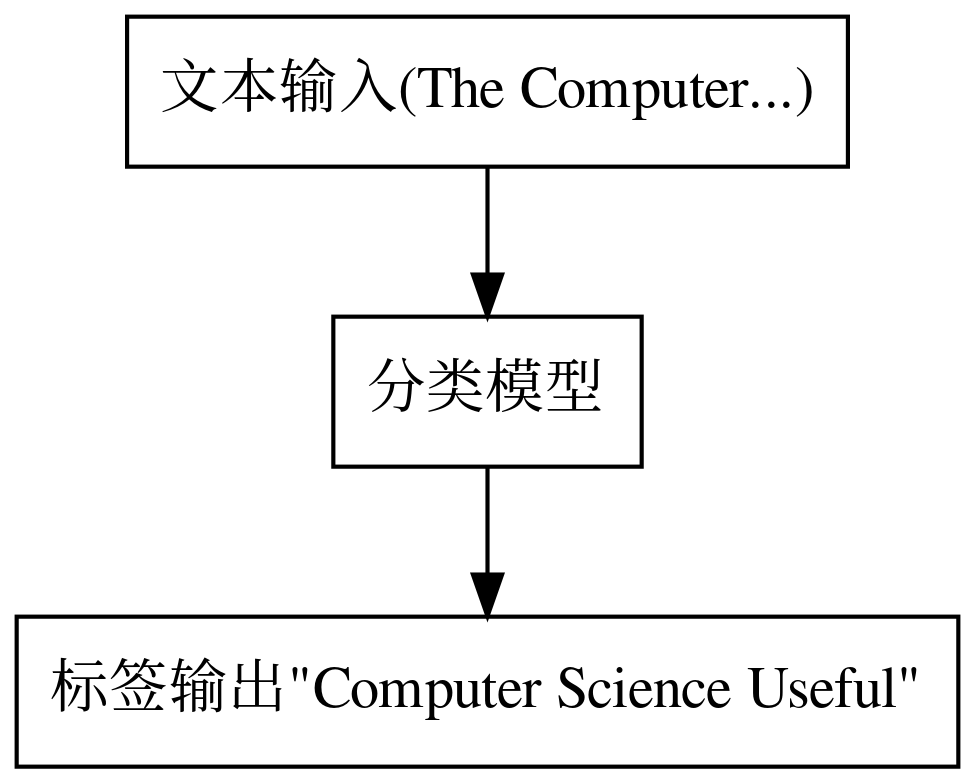
\includegraphics[width=5cm]{./figs/text-classification}
  \caption{文本分类}
  \label{fig:text-classification}
\end{figure}

\subsection{流程}
文本分类的一般化流程如图\ref{fig:textclassification}所示,首先获取到原始数据,通常可使用
API或爬虫。获取到原始数据后就要通常要先进行分词,本文采
用英文文本,分词较为简单,直接取空格分隔即可。分词后,须对每个词进行数据清洗和预处理,取出数字、标点等特殊符号,
去掉停用词、网址、超链接等。获取到“干净”的数据后,使用如TF-IDF、BOW、主题模型等方式对文本
进行特征表示,最后使用提取到的特征,进行分类算法的应用。

\begin{figure}[H]
  \centering
  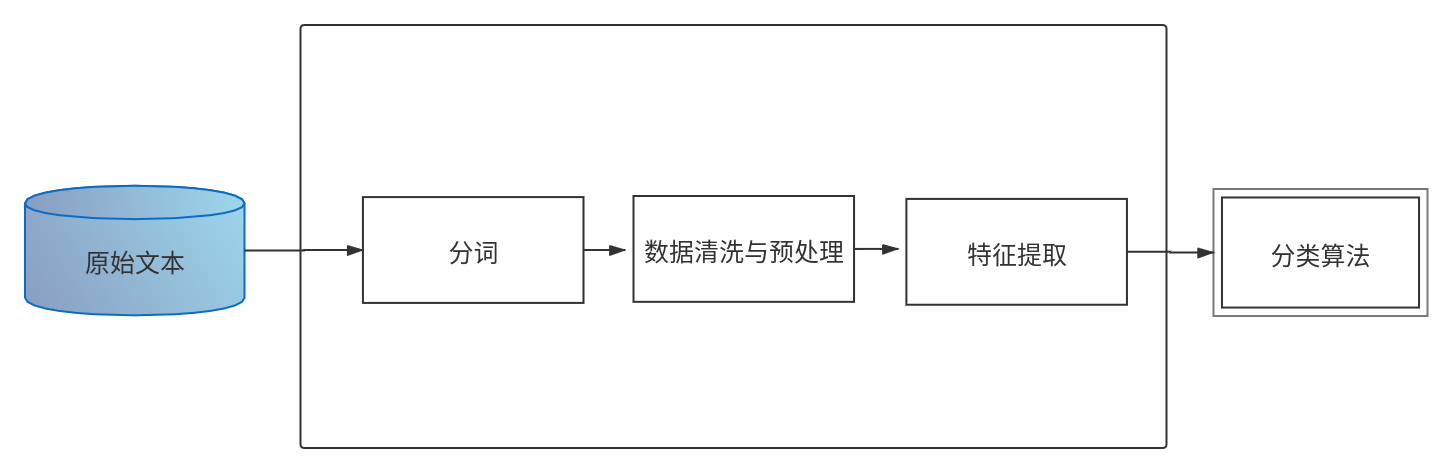
\includegraphics[width=1.0\textwidth]{process}
  \caption{文本分类的一般流程}
  \label{fig:textclassification}
\end{figure}

\section{有监督的短文本分类方法}

\subsection{短文本预处理}
文本预处理是信息检索和文本数据挖掘任务中的重要环节和关键性步骤。一般包括,文档分割、大小写转换
分词、词干提取、词形还原
、去除停用词、规范化、去噪等。

文档分割的步骤通常需要根据文本数据的形式来判断是否需要进行,如果数据集中的每篇文档没有过大且较
为独立,则不需要进行。反之,如果所有的或者大部分数据保存在一个文档中,即需要进行文档切割,
将其分成若干小份,方便后续处理。当然,若多篇文档处于同一个文件中,会有一些特殊的标记区分数
据块,在编程时也很方便去处理。

如果文本是英文字符,则需要将其统一为小写字母,可以降
低字典重复率。

分词,就是将一个句子分成一个个词汇的过程。目的是使得词变成最基础的“数据结
构”,方便后续处理。分词在某种意义上就可以看成是对问题的形式化,将“无结构”的文本数据,
整理成“结构化数据”,方便进行特征表示,分词是所有文本处理类问题形式化的第一步。

词干提取(steming),是将
词语中的变形减少到其“根”的形式的过程。例如将“connect”、“connectedy”以及“connection”都转化
成“connnect”。词干提取能够一定程度上缓解稀疏性问题,在搜索引擎中也常常会发现这个技术,比如
你在Google搜索“deeplearning course”和“deep learning course”,通常你都可以获得正确的结果,
就是因为搜索引擎做了这样的处理。词形还原(lemmatization),目标是删除变形并找到“根”形式。与
词干提取区别在于,词形还原寻找正确的词缀,而词干提取只是在相同的位置做切断。% 例如,
% “trouble”、“troubling”、“troubled”都词形还原会映射为“trouble”,而词干提取只会映射成“troubl”。
下面是词形还原和词形提取的对比图:

\begin{table}[H]                                                                    \begin{singlespace}                                                          
    \centering\caption{词干提取和词形还原对比}\label{tab:level}
    \renewcommand{\arraystretch}{1.5} %控制行高    
    \begin{tabular}{lll}\hline
      Original word & stemmed word & lemmatized word \\  \hline                                                
      \verb|trouble| & troubl & trouble\\                                                   
      \verb|troubling| & troubl &trouble \\                                                 
      \verb|troubled| & troubl & trouble \\                                                 
      \verb|troubles| & troubl & trouble \\
      \verb|troublesome| & troubl & trouble \\      
      \hline                                                                  
\end{tabular}                                                              
\end{singlespace}                                                            \end{table}               

停用词是一种语言中最常见的、无实际意义的词。例如,英文中的be动词、介词、连词等。去停用词的目的是删除文本中低信息量词对主题词的影响,使得算法对文本内容有更强的辨别性。例如:
\par\hspace{5em}\verb|"The Computer Science is a quite uesful subject."|\par

去停用词后,
\par\hspace{5em}\verb|"Computer Science useful subject"|\par

规范化,例如“\$100”可以表示成“one hundred dollars”,“2morrow”转化成“tomorrow”。去噪,
用于删除文本非正常文本中的字符,如符号和数字等特殊字符,他们会对文本分析产生干扰。例如
hashtag中开头的“\#”,提醒关注的“@”,超文本链接“https”,转发推文的“RT”等都是需要被处理的。% 最
% 后,文本增强,它是考虑使用外部语料库即之前不存在的消息来扩充文本数据,使得文本语义得到增强,
% 从而进一步提高模型的预测能力。

% subsection{语言模型}         
% 在介绍词向量的特征表示之前,我们需要先了解下语言模型。语言模型是统计学在自然语言处理上的应
% 用,它根据语言的上下文建立数学模型,描述当前词相对于整个文本的关系。N-gram模型是最常见
% 的一种语言模型,可以用来判断一个文档的出现是
% 否合理,也就是将文档出现的可能用概率表示出来。在该模型中,单词被映射到高维空间,然后嵌入组
% 合以获取输入句子的固定大小表示,后来用作输入到分类器。然而,由于考虑了短句中的词序,它容易
% 受到数据高维稀疏的影响。N-gram模型使用链式法则来计算文档出现的联合概率:
% \begin{equation}
%   \label{eq:1}                                                                              
% P(w_1,w_2,\ldots,w_n) = P(w_1)P(w_2\mid w_1)P(w_3\mid w_1,w_2) \ldots P(w_n \mid w_1, w_2,                                                                    
% \ldots, w_{n-1})                                                               
% \end{equation}

\subsection{词向量特征表示}
类似于图像像素点,对于计算机来说,文本字符实际上是无法直接被理解的。在解决文本分类问题时,
需先将文本转化成结构化的向量信息,才能继续应用算法进行处理。

最简单的特征表示方法就是词袋模型(Bag-of-Words)\cite{zhang2010understanding},它将所有的语料中出现的单词看成一个词汇表,词汇表的大
小即为向量空间的大小,文本中所有文档的维度都和该词汇表的维度相同,通过统计每个词出现的次数,
当作该词在向量中的权重。通俗的讲,就是将一篇文档看做是词的袋子,里面装着一个个不同的词。显
然,文档被转换为一个个词以后,词和词之间的上下文关系也就丢失了。

TF-IDF(Term Frequency–Inverse Document Frequency)\cite{ramos2003using},频率-逆文档频率,旨在反映单词对集合或语料库中的文档的重要程度。

TF(Term Frequency),表示某个单词出现的次数,即词频。其表达式如\ref{eq:tf}所示:

\begin{equation}
  \label{eq:tf}
  TF(t_i) = \frac{n_{i, j}}{\sum_k{n_{k,j}}}
\end{equation}

其中,$t_i$表示文本中的第$i$个单词,$n_{i,j}$表示该单词在第$j$个中文档中出现的次数,而分母
是整个语料中出现的所有词的出现次数之和。

IDF(Inverse Document Frequency,逆文档频率),是一个词语普遍重要性的度量,IDF的值越大,说
明该单词重要性越高,更具有代表性。某一单词的IDF值可以由总文本数除以包含该单词的文本数,再
对其得到的商求对数,其表达式如\ref{eq:idf}所示:

\begin{equation}
  \label{eq:idf}
  IDF(t_i) = lg{\frac{|D|}{|\{j:t_i \in d_j\}|}}
\end{equation}
其中,|D|为语料库中的文件总数,
$|\{j:t_i \in d_j\}|$包含词语$t_i$的文件数目,如果词语不在数据中,就导致分母为零,因此一
般情况下使用$1+|\{j:t_i \in d_j\}|$。
最后,得到TF-IDF:

\begin{equation}
  \label{eq:tf-idf}
  TF-IDF_{i,j} = TF_{i,j} × IDF_{i}
\end{equation}

TF-IDF本质上基于词袋模型。

 \subsection{主题模型}           
主题模型是一种基于概率的非监督聚类统计模型,它通过挖掘文档的隐含语义结构(Latent Semanmitc Structure)
,对文档进行分析。不同于传统的语言模型,只考虑文档在空间上的维度,而引入主题的概念,实现文
档在主题空间上的表示。主题模型在文本挖掘问题中的应用十分广泛,其中最著名的就是David Blei提
出的LDA(Latent Dirichlet Allocation)主题模型\cite{blei2003latent}。

LDA是一种生成模型,假设整个语料库一共包含K个主题,每个主题z都被表示成一个词典V上的一元语言模型$\vartheta_{z}$,即词典上的一个多项
式分布。我们进一步假设每个文档对于这个主题有一个文档特定的多项式$\varPhi_{d}$。那么,文档的生成
过程如图\ref{fig:lda}:

\begin{figure}[H]
  \centering
  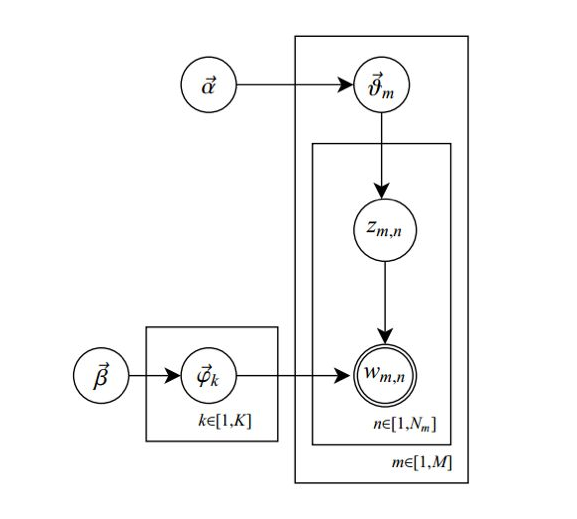
\includegraphics[width=10cm]{./figs/lda.png}
  \caption{LDA主题模型}
  \label{fig:lda}
\end{figure}

其中,$N_m$表示文档中词语的数量,M表示文档的总数量,K表示主题数,$\vartheta$表示文档与主题
之间的多项式分布,$\varphi$表示主题和主题词之间的多项式分布
,$\alpha$和$\beta$分别是$\vartheta$和$\varphi$的
Dirichlet先验参数,$Z_{m,n}$表示词语的主题分布,$w_{m,n}$表示生成的词。生成文档的步骤如下:
\begin{itemize}
\item 从参数为$\alpha$的Dirichlet分布中采样生成主题的多项式分布$\varphi$,
\item 从主题的多项式分布$\varphi$中采样生成第j个主题词$z_{i,j}$
\item 从参数为$\beta$的Dirichlet分布中采样生成主题$z_{i,j}$对应词语的多项式分布$\varphi_{k}$
\item 从词语的多项式分布$\varphi_{k}$中采样生成最终词语$w_{i,j}$
\end{itemize}

 % \subsection{文本扩展技术}
 % 常见的文本扩展技术有基于主题模型(Topic Model)的短文本扩展技术以及基于外部语料库的文本扩
 % 展技术。
 
\section{有监督的短文本数据流分类方法}
% 本小节将介绍有监督的短文本数据流分类方法,需要用到的基础理论和技术, 分别数据流定义、支持向
% 量机、集成分类方法 、相似性度量、分类效果衡量指标
% 以及概念漂移。

\subsection{数据流定义}
数据流是由随着时间推移到达的大量的、连续的数据项组成的序列\cite{陈火旺A}。若令t表示某一时刻,
则数据流可形式化地表示为$D=\{d_1,d_2,…,d_{t-1},d_{t},d_{t+1},…\}$其中,$d_t=\{x_{t},y_{t}\}$,
$x_{t}$为第i个属性值,$y_{t}$表示该属性值对应的类标签。

数据流具备动态实时、持续到达、易变、高维稀疏等特点。正是由于这些特点,使得数据流无法将传统的机器学习算法如决策树、支持向量机、贝叶斯等算法直接应用,这给数据流分析带来了挑战。

\subsection{支持向量机}
支持向量机(Support Vector machine),是一种有监督(Supervised Learning)
\cite{russell2002artificial} 的二元分类器。首次
由Vapnik等人1964年提出\cite{Vapnik1964A},而后又经过多次优化与提高,使其可以应用于多元分类
任务\cite{Hsu2002A}。其基
本模型定义为特征空间上的间隔最大的线性分类器,即在样本空间中找到一个超平面,使得它可以最大
分隔两个类。

\begin{figure}[H]
  \centering
  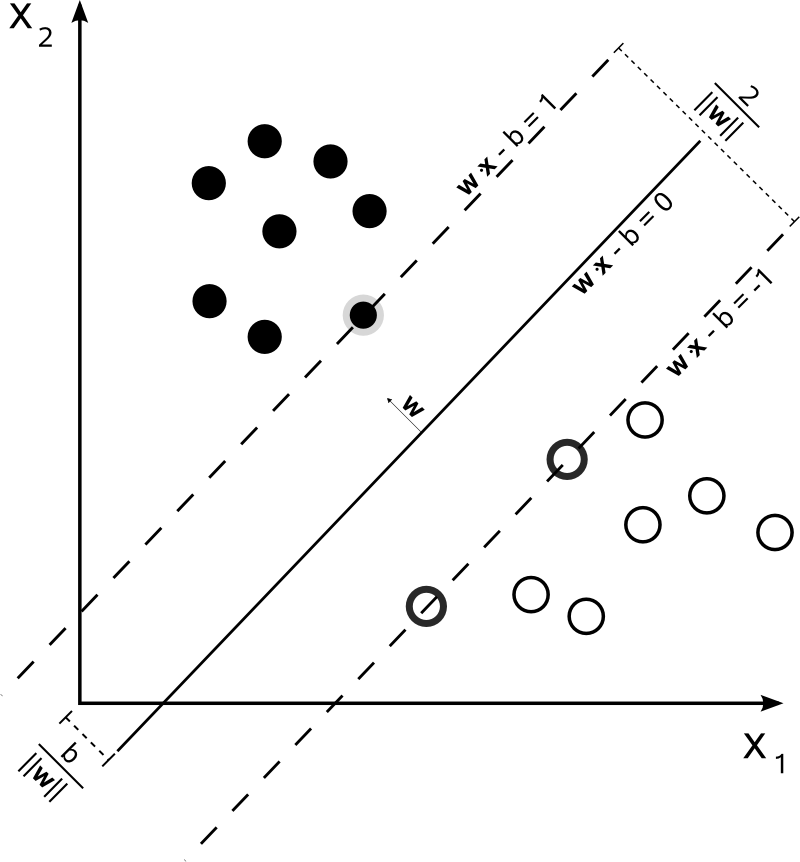
\includegraphics[width=10cm]{./figs/svm.png}
  \caption{支持向量机}
  \label{fig:svm}
\end{figure}

如图\ref{fig:svm}所示,其中$wx-b=1$和$wx-b=-1$表示两条支持向量,中间的$wx-b=0$即为找到的超
平面。对于这样一个二维数据集来说,最优超平面的寻找较为简单,但实际使用中的数据集往往远超二维,
对于这样的高维数据来说,不一定都是线性可分的,因此想要找到最佳超平面的就需要借助核函数,将样本空间映射到更高维的空间,
使得数据变得线性可分,以方便更好的进行样本分离。通常,核函数的选择也会直接影响到模型的分类性能,故如何选择更好的
核函数也很重要,下面是几种SVM常用的核函数:

\begin{table}[H]                                                                    \begin{singlespace}                                                          
    \centering\caption{SVM核函数对比}\label{tab:level}
    \renewcommand{\arraystretch}{1.5} %控制行高    
    \begin{tabular}{llp{6cm}}\hline
      核函数 & 计算公式 & 描述 \\  \hline                                                
      \verb|线性核函数| & $K(x_i,x_j)=x_i^Tx_j$ & 其中,K为半正定核矩阵,适用于线性可分的数据,速度较快\\                                                   
      \verb|多项式核函数| & $K(x_i,x_j)=(x_i^Tx_j)^d$ &  其中,$d \geq 1$\\
      \verb|高斯核函数| & $K(x_i,x_j)=exp(-\frac{{||x_i-x_j||}^2}{2\sigma^2})$ & 其中,$\sigma
                                                                                 \geq 0$
                                                                                 为高斯核
                                                                                 的带宽 \\
      \verb|拉普拉斯核函数| & $K(x_i,x_j)=exp(-\frac{||x_i-x_j||}{\sigma})$ & $\sigma
                                                                                 \geq 0$ \\
      \verb|Sigmoid 核函数| &  $K(x_i,x_j)=tanh(\beta x_i^Tx_j+\theta)$ & 其中, $tanh$为双曲正切函数,$\beta>0$,$\theta>0$ \\            
      \hline                                                                  
\end{tabular}                                                              
\end{singlespace}
\end{table}

\subsection{集成方法}
集成方法也叫集成学习(Ensemble Learning) ,不同于决策树、支持向量机等分类器的是,它不是一
个新的分类算法,而是一种机器学习范式。集成方法的思想是,通过训练多个分类模型,将所有的模型
综合起来得到更好的预测结果。大量的实践证明它能够带来更高的准确率和更强的鲁棒性。

在快速数据流中,分类模型通常不能稳健地建立。因此,采用集成分类方法,通过组合不同的分类器可
以使模型更加健壮。另一方面,数据以流的形式出现, 在机器的内存中直接容纳大量流数据是不切
实际的,而且通常是不可行的。因此在这种情况下,可以借助集成模型,连续更新并通过使用最近一批
数据进行再训练来增量地训练预测模型。bagging和boosting是两种最常见的集成方法\cite{oza2005online}。

Street等\cite{street2001streaming}将集成应用到文本数据流分类中,思想是以块为单位顺序读取训
练数据,在当前块学习分类器,并在下一个块上进行评估,缺点是没有考虑到概念漂移。wettschereck
等\cite{wettschereck2003mining}设计了处理概念漂移的集成方法,它可以有效地发现数据流的迁移,该方法中,数据流被分割成块,每个块上都有多个分类器,并且最终的分类权值通过每个块上函数计算。kotler,zhang等\cite{kotler2003dynamic,zhang2009mining}也都使用这种模型加权或模型选择方法,来确保概念漂移数据流分类获得更好的
精度。

\subsection{概念漂移}
概念漂移(Concept Drift)\cite{widmer1996learning} 是指在非平稳的环境中,数据分布会随着时
间而变化,改变数据流上下文中的隐含信息,从而产生概念漂移现象。数据流分类的目标是训练分类
器,建立一个类标签和特征之间的函数关系。而概念漂移是数据流分类中最早出现的,也是比较棘手的问题之一。
  
一个典型的示例是用户对新闻信息流兴趣的变化,虽然新闻文档的分发通常保
 持不变,但该用户感兴趣的新闻文档的条件分布却发生了变化。

最通用的解决思路就是通过历史数据分析,抽象出数                             据的模式随时间变化的规律,其中可能包括若干趋势和周期的混杂信号。但多数情况下,随时间的变化
有很强的随机性,这很难做到。

在过去的一段时间里,与概念漂移有关的学习的研究越来越多,并且已经开发了许多漂移感知的自适应学习算法。
自适应学习是指在运行过程中在线更新预测模型以对概念漂移做出
反应。Tsymbal等人在2004年发表的概念漂移综述文章\cite{tsymbal2004problem}对该问题给出了相对较全的定
义,并附出了当时相关工作;kuncheva\cite{kuncheva2004classifier,kuncheva2008classifier}将集
成学习技术应用于概念漂移检测上。maloof等提出了归纳规则学习算法\cite{maloof2010aq};
shirakawa等基于语
义扩展的方法\cite{shirakawa2015wikipedia}以及phan等基于主题模型的方法\cite{phan2010hidden}
下面将主要将描述自适应学习算法的特点。

自适应学习算法可以看作是先进的增量学习算法,能够随着时间的推移适应生成数据的过程。假设数据满足独立同分布,首先建立静态的基模型作为评估基准,默认随时间推移自变量和因变量的映
射关系一致,在通过这个模型检测是否存在概念漂移。
在训练之前,根据时序给样本不同的权重,时间越新的样
本权重可以给大一点,越老的数据可以减少权重                                      。
然后定期的加入新数据更新模型。在加入新数据的时候,也可以进一
步筛选出最适合的样本进行重新训练,得到更加适合的模型。

%\subsection{相似性度量}
%\subsection{分类效果衡量指标}

\section{平台开发相关技术}
本文处实现相关算法外,还构建了一个可视化的数据挖掘平台。本小节将介绍搭建数据挖掘平台需要用
到的Web相关技术,其中包括Django框架、MongoDB数据库和Echart可视化图标的相关介绍。
\subsection{Django框架}
Django 是一个高级的 Python 网络框架,通过自动化或简化Web开发的常见任务,快速开发安全和可维
护的网站。Django让代码编写者只需要专注于编写应用程序,网站开发中麻烦的部分已经被封装
完成,无需重新开发。
 Django开发的应用有如下几个优点
\begin{itemize}
\item 具有很好的完备性,几乎提供Web开发所需要的所有模块;
\item 可以构建几乎任何类型的后端,处理各种格式(HTML、JSON、XML)的数据;
\item 重视安全问题,例如常见的SQL注入、CSRF攻击等都有很好的防护;
\item 采用类MVT的设计原则,易于扩展性、可维护性高;
\item 灵活性高,采用Python编写,天生具备跨平台的能力;
\end{itemize}

Django的核心是一组高效协同工作的库,涵盖了Web开发的各个方面,其中包括:ORM对象关系映射器,该库知道数据库的结构,代码的结构,并且无需重复的手写SQL语句就能弥合它们之间的鸿沟。一组HTTP
库,它们知道如何解析传入的Web请求,并返回标准格式给用户。URL路由库,可让您准确定义所需的
URL并将它们映射到代码的适当位置。一个视图系统, 用于处理请求。 
Template模板系统,使用它编写混合模板语言的HTML代码,接受后端传来的数据,在网页中显示表单并
处理用户提交的数据。图\ref{fig:django}是Django的整体框架图。

\begin{figure}
  \centering
  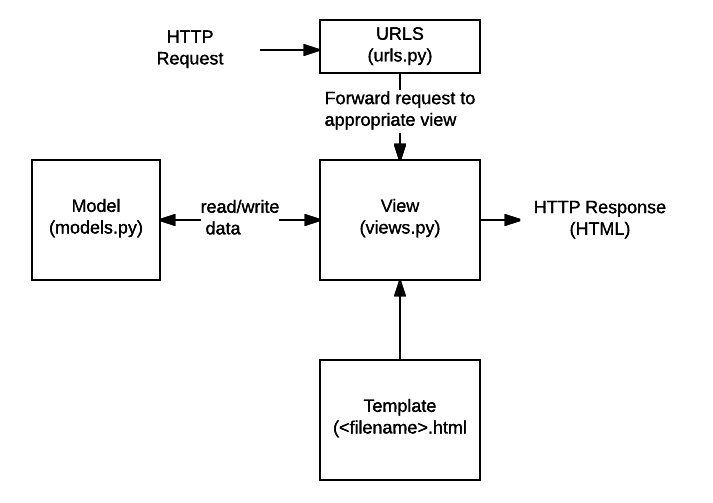
\includegraphics[width=10cm]{django}
  \caption{Django MVT设计框架图\cite{mozilla.org}}
  \label{fig:django}
\end{figure}

\subsection{MongoDB}
MongoDB是一种NoSQL数据库,NoSQL被称作“Not Only SQL”,在数据爆炸的今天使用十分广泛。
几年前,应用程序通常只拥有数千个用户到上万个用户,而现在流行的APP如“新浪微博”、
“Wechat”的用户都数以亿计,并且每年365天,每天7*24小时处于连接状态。传统的关系型数据库在处
理少量数据时它们具有良好的性能。但处理当下信息大爆炸时代互联网,多媒体和社交网络的海量数据,
使用传统的关系数据库效率低下。为了克服这个问题,引入了“ NO SQL”一词。 NoSQL术语由Carlo
Strozzi于1998年创造,指非关系数据库。MongoDB就是最流行的NoSQL数据库之一。

MongoDB采用C++语言编写的,一个开源的分布式文件存储数据库系统。MongoDB将所有的数据都是为文
档,文档数据结构表示方式采用Key-Value的形式,类似于JSON。

MongoDB主要特点如下:
\begin{itemize}
\item 可实现传统数据库能实现的所有操作;
\item 采用面向文档的设计模式,操作更加简单;
\item 由于存储特点,可应用于分布式计算;
\item 读取效率相比传统数据库更高;
\item 丰富的查询表达式。可轻易查询文档中内嵌的对象及数组;
\item 支持多种编程语言,安装便捷;

  图\ref{fig:mongodb}是MongoDB的架构:
  \begin{figure}
  \centering
  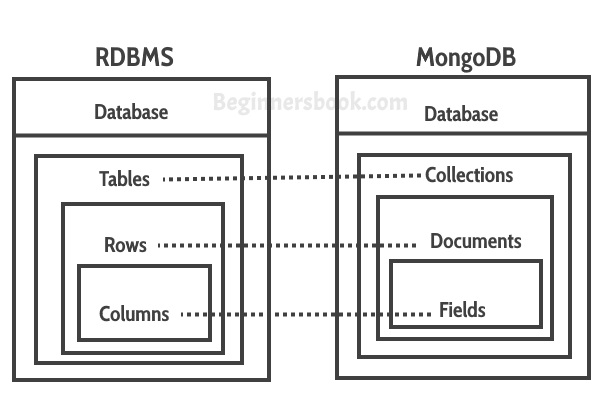
\includegraphics[width=10cm]{mongodb}
  \caption{RDBMS vs MongoDB\cite{beginnersbook.com}}
  \label{fig:mongodb}
\end{figure}
\end{itemize}

\subsection{Echart}
ECharts(Enterprise Charts)是国产的应用于浏览器的可视化工具箱。使用简单的Javascript语法,就可以完成对数据的操作,同时画出美观的图表。

\section{本章小结}
本章节详细介绍了本文研究问题相关的技术和理论,其中包括大数据分析的基本流程,讨论了文本分类常用
的技术手段。并对有监督的文本分类方法和有监督的文本数据流分类方法分别做了理论介绍,大致包括文本
预处理、语言模型、词特征表示、主题模型、数据流定义、支持向量机、集成分类方法、概念漂移现象
等。通过阅读本章节,读者可以对本文研究的背景知识有了大致的了解。
 % 相关工作概述
\chapter{基于概念漂移检测的短文本数据流分类算法设计}

% \section{引言}                  
本文提出一种基于概念漂移检测的短文本数据流分类算法,用于对短文本数据流进行隐含主题的跟
踪。该方法采用集成学习,将时序的文本数据流进行分块,针对每个块训练一个基础SVM分类器,并根
新旧据块之间的语义距离判断是否发生概念漂移,结合分配给每个分类器的权重,动态地更新模型池中
的基分类器,使得模型池中始终保持恒定数量的分类器。对于新到来的未知标签的数据块,采用该集成
模型进行预测和分析,这就是本文提出的主题跟踪的算法基础。

% 接下来,本章会从问题定义开始,详细
% 介绍如何设计一个高效可用的集成模型。

\section{框架设计}

% 在这个部分,对于短文本数据流集成分类算法进行了形式化。
假定数据流由N个数据块组成,命名为$D = \{
D_1,  D_2,  …… , D_N \}$ ,每个数据块包含一些短文本,命名为$D_i = \{ d_1, d_2, …… , d_n \}$,
其中n表示第i个数据块的短文本数目。
通常,每个文档都能被表示成一个向量空间,命名为$d_j = \{ (v_x, v_y)  |  v_x \in R^M, v_y
\in Y\}$,其中$R^M$表示一个文档空间,Y表示该文档的标签,M表示维度。

为解决短文本数据流的稀疏性问题,本文使用Wikipedia作为外部语料库对短文本进行语义扩展,缓解
该问题,扩展后的数据块表示为$D_i^{'}=\{d_j^{'}\}_{j=1}^{|D_i|}$。然后使用BTM主题模型将扩展
后的数据块特征表示K维的主题分布,记作$D_i^{''}=\{d_j^{''}\}_{j=1}^{|D_i|}$。


最终,本文的目标是训练一个动态的集成模型$f : E_{\sum{D_i}}
\rightarrow Y$,将特征向量映射到标签上,以适应未知的短文本数据流并且发现短文本数据流中存在的概念漂移现象。

为了高效地处理短文本数据流分类问题,该方法的框架是由H个基分类器组合,构建一个集成分类模型 $E = \{ f_1, f_2, ……,f_h \}$。当新的数据块$d_j$来的时候,集成分类模型通过公式\ref{eq:1}赋予$d_j$一个类标签$y^*$。
  \begin{equation}
    \label{eq:predict}
    y^* = argmax_{y \in Y}P(y|d, E)     
  \end{equation}
    
其中后验概率$P(y|d, E)$是通过K个基分类模型进行加权平均所得,如公式\ref{eq:2}

\begin{equation}
  \label{eq:2}
  P(y|d, E) = \sum_{i=1}^{K}w_iP(y|d, f_i)
\end{equation}

% 在该方法中,每个文档d都可以被表示成一个个词特征向量。为了提取特征向量,需要识别短文本中所
% 包含的词。这涉及到接下来相关的两个重要技术,叫做特征表示和短文本扩展。

%通过统计得出,实验数据中短文本所占比
% 例达95,因此,我们仅用特征词特征空间来表示短文本,记作$ V_d = \{ T \}$。

图\ref{fig:shorttextclass}是整个算法的流程:

\begin{figure}[htb]
  \centering
  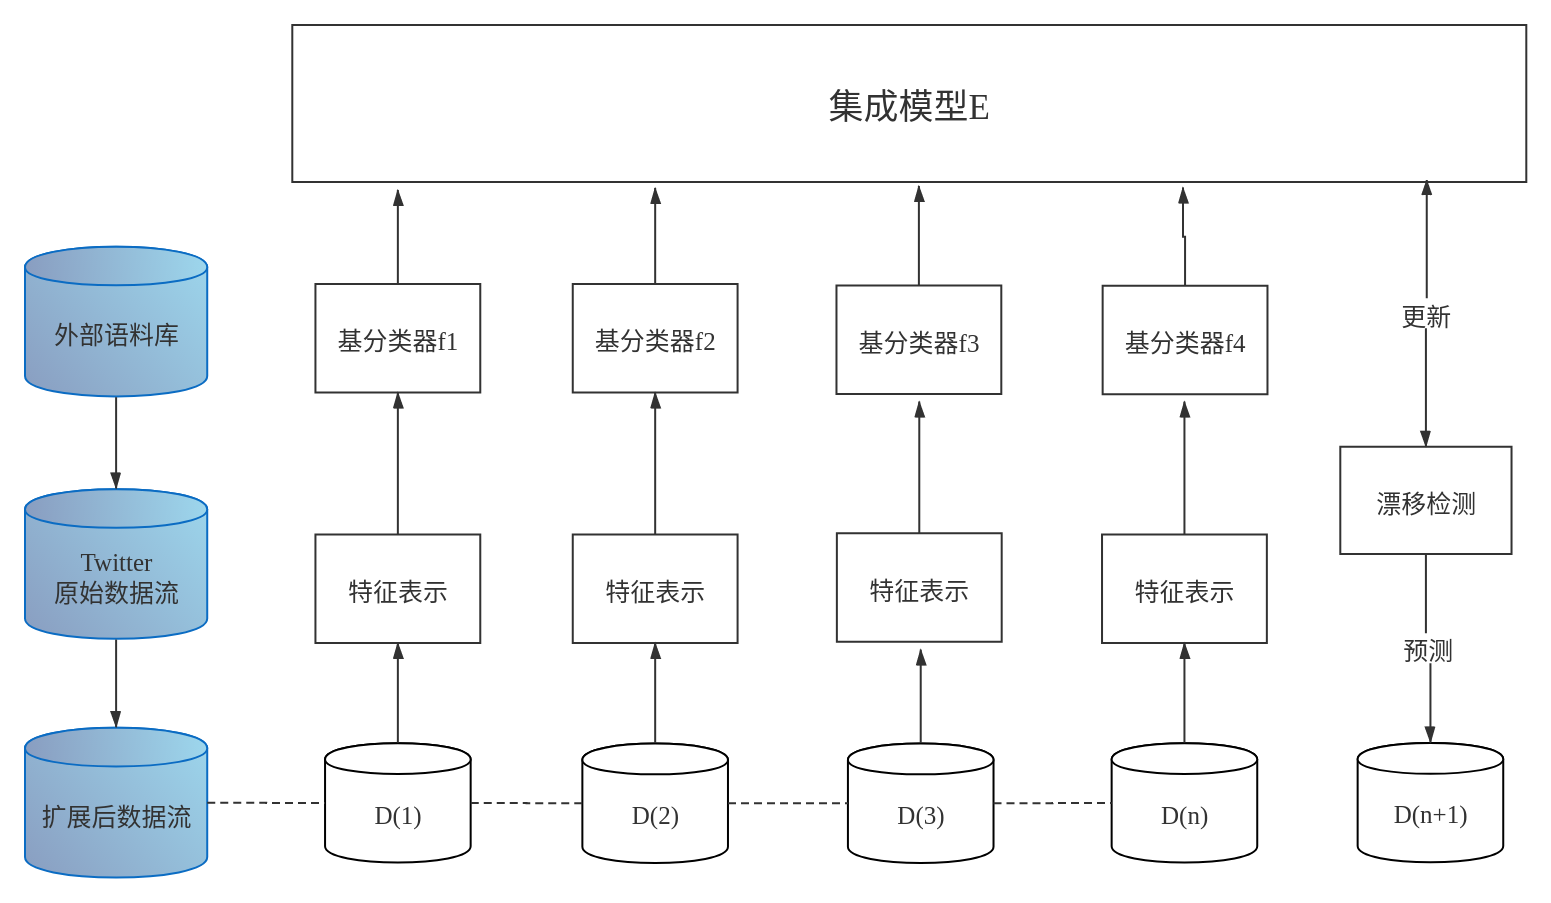
\includegraphics[width=1.0\textwidth]{shorttext}
  \caption{短文本数据流分类流程图}
  \label{fig:shorttextclass}
\end{figure}

% \section{数据预处理}

\section{数据采集与预处理}
本课题的实验数据来自Twitter,使用Twitter官方提供的“关键字搜索”API进行自动化采集。一共收集
了从2011年11月份到2013年1月份的5个类别的共约181万条数据。图\ref{tab:number}是每个类别的数量,图\ref{tab:exp}是数据实例。

\begin{table}[H]                                                                    \begin{singlespace}                                                          
    \centering\caption{每个类别的数量}\label{tab:number}
    \renewcommand{\arraystretch}{1.5} %控制行高
    \begin{tabular}{p{2.5cm}p{2cm}}\hline                                                        标签    
      & 数量 \\ \hline                                                
      \verb|arsenal| & 515017 \\                                                   
      \verb|blackfriday| & 137767 \\
      \verb|smartphone| & 401361 \\
      \verb|chelsea| & 647879 \\
     \verb|obama| & 112155 \\ \hline                                     
    \end{tabular}                                                                                       
  \end{singlespace}
\end{table}

\begin{table}[H]                                                                    \begin{singlespace}                                                          
    \centering\caption{类别实例}\label{tab:exp}
    \renewcommand{\arraystretch}{1.5} %控制行高
    \begin{tabular}{p{2.5cm}p{12.5cm}}\hline                                                        标签
      & 实例 \\ \hline                                                
      \verb|arsenal| & why arsenal fans always proud of their history, are they living in past? \\                                                   
      \verb|blackfriday| &  BeachBody's having Black Friday deals too! Check out these
                           great deals! http://t.co/NphfZ5Xu \\
      \verb|smartphone| & @MsEmeraldEyez ok got you posted up here: http://t.co/jzPIpstF feel special ur the 1st one :)            \\
      \verb|chelsea| &   @chelseaaaakay god fucking damnit Chelsea you don't get it.                                                                                \\
     \verb|obama| &    I love these auto-add programs, b/c I just got an e-mail saying that "Barack Obama is now following you on Twitter!" How cool is that?                                                                                                                                       \\ \hline                                     
    \end{tabular}                                                              
  \end{singlespace}                                                            \end{table}               

为了有效挖掘数据隐藏的主题信息,需要进行数据预处理,操作步骤如下:

\begin{enumerate}
\item
首先将文本所有的字母变成小写,并借助正则表达式去掉文本中的email、以@开头的词、换行符、网址
链接、标点符号等特殊字符;
\item  加载停用词列表,删除文本中的停用词,并对每个单词进行词干提取和词形转换;  
\item 将文本字符串分词,生成词汇列表;
\end{enumerate} 

图\ref{tab:before}和图\ref{tab:after}是数据预处理前后对比:

\begin{table}[htb]                                                                    \begin{singlespace}                                                          
    \centering\caption{处理前}\label{tab:before}
    \renewcommand{\arraystretch}{1.5} %控制行高
    \begin{tabular}{p{13.5cm} p{2.5cm}}\hline
      文本 & 标签 \\ \hline                                                
      @MsEmeraldEyez ok got you posted up here: http://t.co/jzPIpstF feel special ur the 1st one :)  & smartphone \\
      Useful Smartphone Apps  http://t.co/2WDnIIgg  & smartphone \\
      New post: Consumers face many more tablet choices this holiday season http://t.co/s76GLU5R  & smartphone \\
      Iphone 5 is the fastest smartphone, beat galaxy s3 and others! http://t.co/gScgoW95  & smartphone \\
      Yeah..bibinyagan ko ang bgong tablet pc... :-)  & smartphone \\
      \end{tabular}                                                              
  \end{singlespace}
\end{table}               

\begin{table}[ht]                                                                  \begin{singlespace}                                                          
    \centering\caption{处理后}\label{tab:after}
    \renewcommand{\arraystretch}{1.5} %控制行高
    \begin{tabular}{p{13.5cm} p{2.5cm}}\hline
      文本 & 标签 \\ \hline                                                
      msemeraldeyez ok got post http t co jzpipstf feel special ur 1st one  & smartphone \\
      use smartphone app http t co 2wdniigg  & smartphone \\
      new post consum face mani tablet choic holiday season http  & smartphone \\
      iphon fastest smartphon beat galaxi s3 http t co gscgow95 & smartphone \\
      yeah bibinyagan ko ang bgong tablet pc  & smartphone \\
      \end{tabular}                                                              
  \end{singlespace}
\end{table}               


\section{短文本扩展}
由于短文本数据缺乏足够的语义信息,本节借助短文本扩展技术,对缺乏短文本的数据进行语义扩展,
缓解特征高维稀疏的问题。短文本扩展需要用到外部语料库,而语料库的质量将对实验结果有着较大的
影响。本文采用的语料库来自Wikipedia。Wikipedia是最权威的在线百科,噪音数据较少,并且内容丰
富、有多种类型的短文本。借助Wikipedia官方提供的工具JwikiDocs,通过在短文本数据流中提取到的关键词进行检索,可以很方
便地获取到数据。

同样,需要对这些获取到的数据进行相关数据预处理和清洗。然后,就可以开始进行短文本扩展了。首
先使用LDA(Latent Dirichlet Allocation)主题模型,提取语料库中的主题信息,将得到的模型记作$M_{lda}$。然后,将模型$M_{lda}$应用到每个数据块中进行主题推断(Topic Infer)\cite{phan2010hidden},
获得这些数据块中短文本的主题分布。最后再根据该主题分布将语料库中具有相同分布的词添加到短文
本中,就实现了对文本的扩展。

\section{特征表示}
完成对短文本的扩展后,借助另一种主题模型BTM(Biterm Topic Model),将扩展后的短文本表示为
主题分布。LDA(Latent Dirichlet Allocation)主题模型依
靠的是词袋模型的假设,在对短文本进行表示时,容易得到高维稀疏的矩阵,影响算法的运算效率和精度。相比之下,BTM主题模型采用词对共现的方式进行建模,就在一定程度上避免了这个问题,因此,BTM主题模型更加适用于短文本。图\ref{fig:btm}是BTM模型的生成过程。

\begin{figure}[ht]
  \centering
  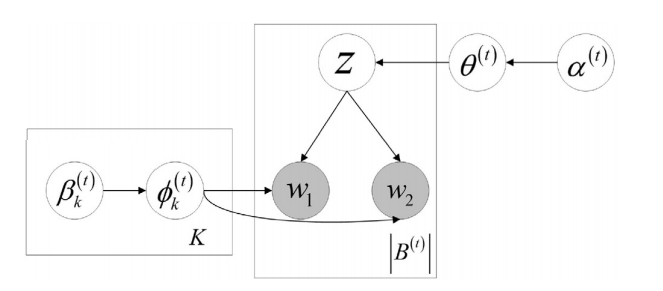
\includegraphics[width=10cm]{./figs/btm.png}
  \caption{$t^{th}$时间片内的BTM主题模型}
  \label{fig:btm}
\end{figure}

其中,K表示主题数,$B^{t}$表示由$\{w_1,w_2\}$组成的词对集合,称作一个biterm。
$\alpha^{(t)}$和$\beta_{k}^{(t)}$分别是 $\varphi^{(t)}$和$\theta^{(t)}$的Dirichlet分布的先
验参数,$\theta^{(t)}$是K维的文档-主题多项式分布,$\varphi^{(t)}$是W维的主题-词分布; $Z_{m,n}$表示词语的主题分布,$w_1$和$w_2$是在该分布下取样生成的词;
下面是BTM模型的生成步骤:
 
\begin{center}
  \begin{itemize}
\item Draw a topic distribution in the $t^{th}$ time slice $\theta^{(t)}~Dirichlet(\alpha^{(t)})$;
\item For each topic k from K topics:\\
        (a) Draw a word distribution of topic in the $t^{th}$ time slice $\varphi^{(t)}~Dirichlet(\beta^{(t)})$
      \item For each biterm $b_j = {w_{j,1},w_{j,2}} \in B^{(t)}$:\\
        (a) Draw a topic $z_j ~ Multinomial(\theta^{(t)})$;\\
        (b) Draw words $w_{j,1},w_{j,2} ~ Multinomial(\varphi_{z_{j}}^{(t)})$;\\
 \end{itemize}
\end{center}

由于短文本是以流的形式传入模型的,本文将流数据按时间顺序进行分块,并设置好块大小。每当数据块来临的时候,即使用BTM算法对块数据进行特征表示,得到块的特征值。本文实验数据总文本数为10000,共5个类别,采用的块大小为1000,BTM主题模型主题数为5,BTM迭代次数100次,借助python第三方库“biterm”,对BTM算法进行了调用,从而得到每个块的特征值。借助BTM模型,对扩展后的数据块$D_i^{'}$进行主题推断,将起表示为一组主题分布,即得到$D_i^{''}=\{d_j^{''}\}_{j=1}^{|D_i|}$,其中$d_j^{''}=\{z_{j,k}\}_{k=1}^K$,,$z_{j,k}$表示$j^{th}$短文本中$k^{th}$主题值。

\begin{table}[htb]
  \begin{singlespace}                                                          
    \centering\caption{BTM主题词提取结果}\label{tab:before}
    \renewcommand{\arraystretch}{1.5} %控制行高
    \begin{tabular}{l}\hline
Topic 0 | Top words = black friday chelsea mobile obama arsen \\
Topic 1 | Top words = obama presid bush czar blackberri smartphone \\
Topic 2 | Top words = chelsea arsen phone intern free obama \\
Topic 3 | Top words = win day smartphon chelsea tablet liverpool \\ 
Topic 4 | Top words = tangan jam murah hdmi ic 20 \\ 
\hline                                                      
     \end{tabular}                                                              
  \end{singlespace}
\end{table}               

% 我们使用Gibbs采样的方法,获得每个时间片$t^{th}$的文档-主题分布
% $\theta{(t)}=\{\theta_k^{(t)}\}_{k=1}^{K}$和主题-词分布
% $\varphi{(t)}=\{\varphi_k^{(t)}\}_{k=1}^{K}$,其中
% $\varphi_{k}=\{\varphi_{k|w}^{t}\}_{w=1}^{W}$。若每个短文本d中可生成$N_b$个无序词对,即
% $\{b_j^{d}\}_{j=1}^{N_b}$,其中$b_j^{(d)}=(w_{j,1}^{(d)},w_{j,2}^{(d)})$,则短文本的主题
% 为k的概率可以表示为:

% % \ref{eq:pkd}:

% \begin{equation}
%   \label{eq:pkd}
%  P(k|d) = \sum_{j=1}^{N_b} P(k|b_j^{(d)})P(b_j^{(d)}|d) 
% \end{equation}

% 其中,$P(k | b_j^{(d)})$表示短文本d中第j个词对是主题k的概率,$P(b_j^{(d)} | d)$表示短文本d中包
% 含词对$b_j^{(d)}$的概率。

% \subsection{主题跟踪}

\section{概念漂移检测}
在短文本数据流分类中,主题随着时间的推移发生会变化从而产生概念漂移。概念漂移会严重影响
到模型的预测精度,因此解决该问题对本模型十分重要。本文通过主题的分布
来检测检测概念漂移。


每当新的数据块来的时候,我们通过计算该数据块中的每个短文本和当前数据块的语义距离,再计算均
值来判断新数据块是否发生了概念漂移,公式\ref{eq:dist1}如下:

\begin{equation}
  \label{eq:dist1}
       dist(D_{i+1}^{''},D_{i}^{''})=1 / |D_{i+1}|\sum_{j=1}^{|D_{i+1}|}dist(d_j^{''},D_i^{''})
\end{equation}

其中,$dist(d_j^{''},D_i^{''})$为短文本和当前数据块之间的距离,首先根据类分布,将当前数据
块分割成大小为C的簇,记作$\{I_c\}_{c=1}^{C}$,其中$I_c=\{d_i^{''}\}_{I=1}^{|I_c|}$,
$|I_c|$表示$c^{th}$类簇中的短文本数,再计算短文本和所有类簇之间的语义距离,选择语义
距离最小的值表示该短文本与数据块之间的语义距离,如公式\ref{eq:dist2}:

\begin{equation}
  \label{eq:dist2}
  dist(d_j^{''}, D_i^{''})=min dist(d_j^{''},I_c)
\end{equation}

其中,$dist(d_j^{''},I_c)=1/|I_c|\sum_i^{|I_c|}dist(d_j^{''},d_l^{''}), d_I^{''} \in I_c $。图\ref{fig:concept-drift}是本算法的流程图。

\begin{figure}[H]
  \centering
  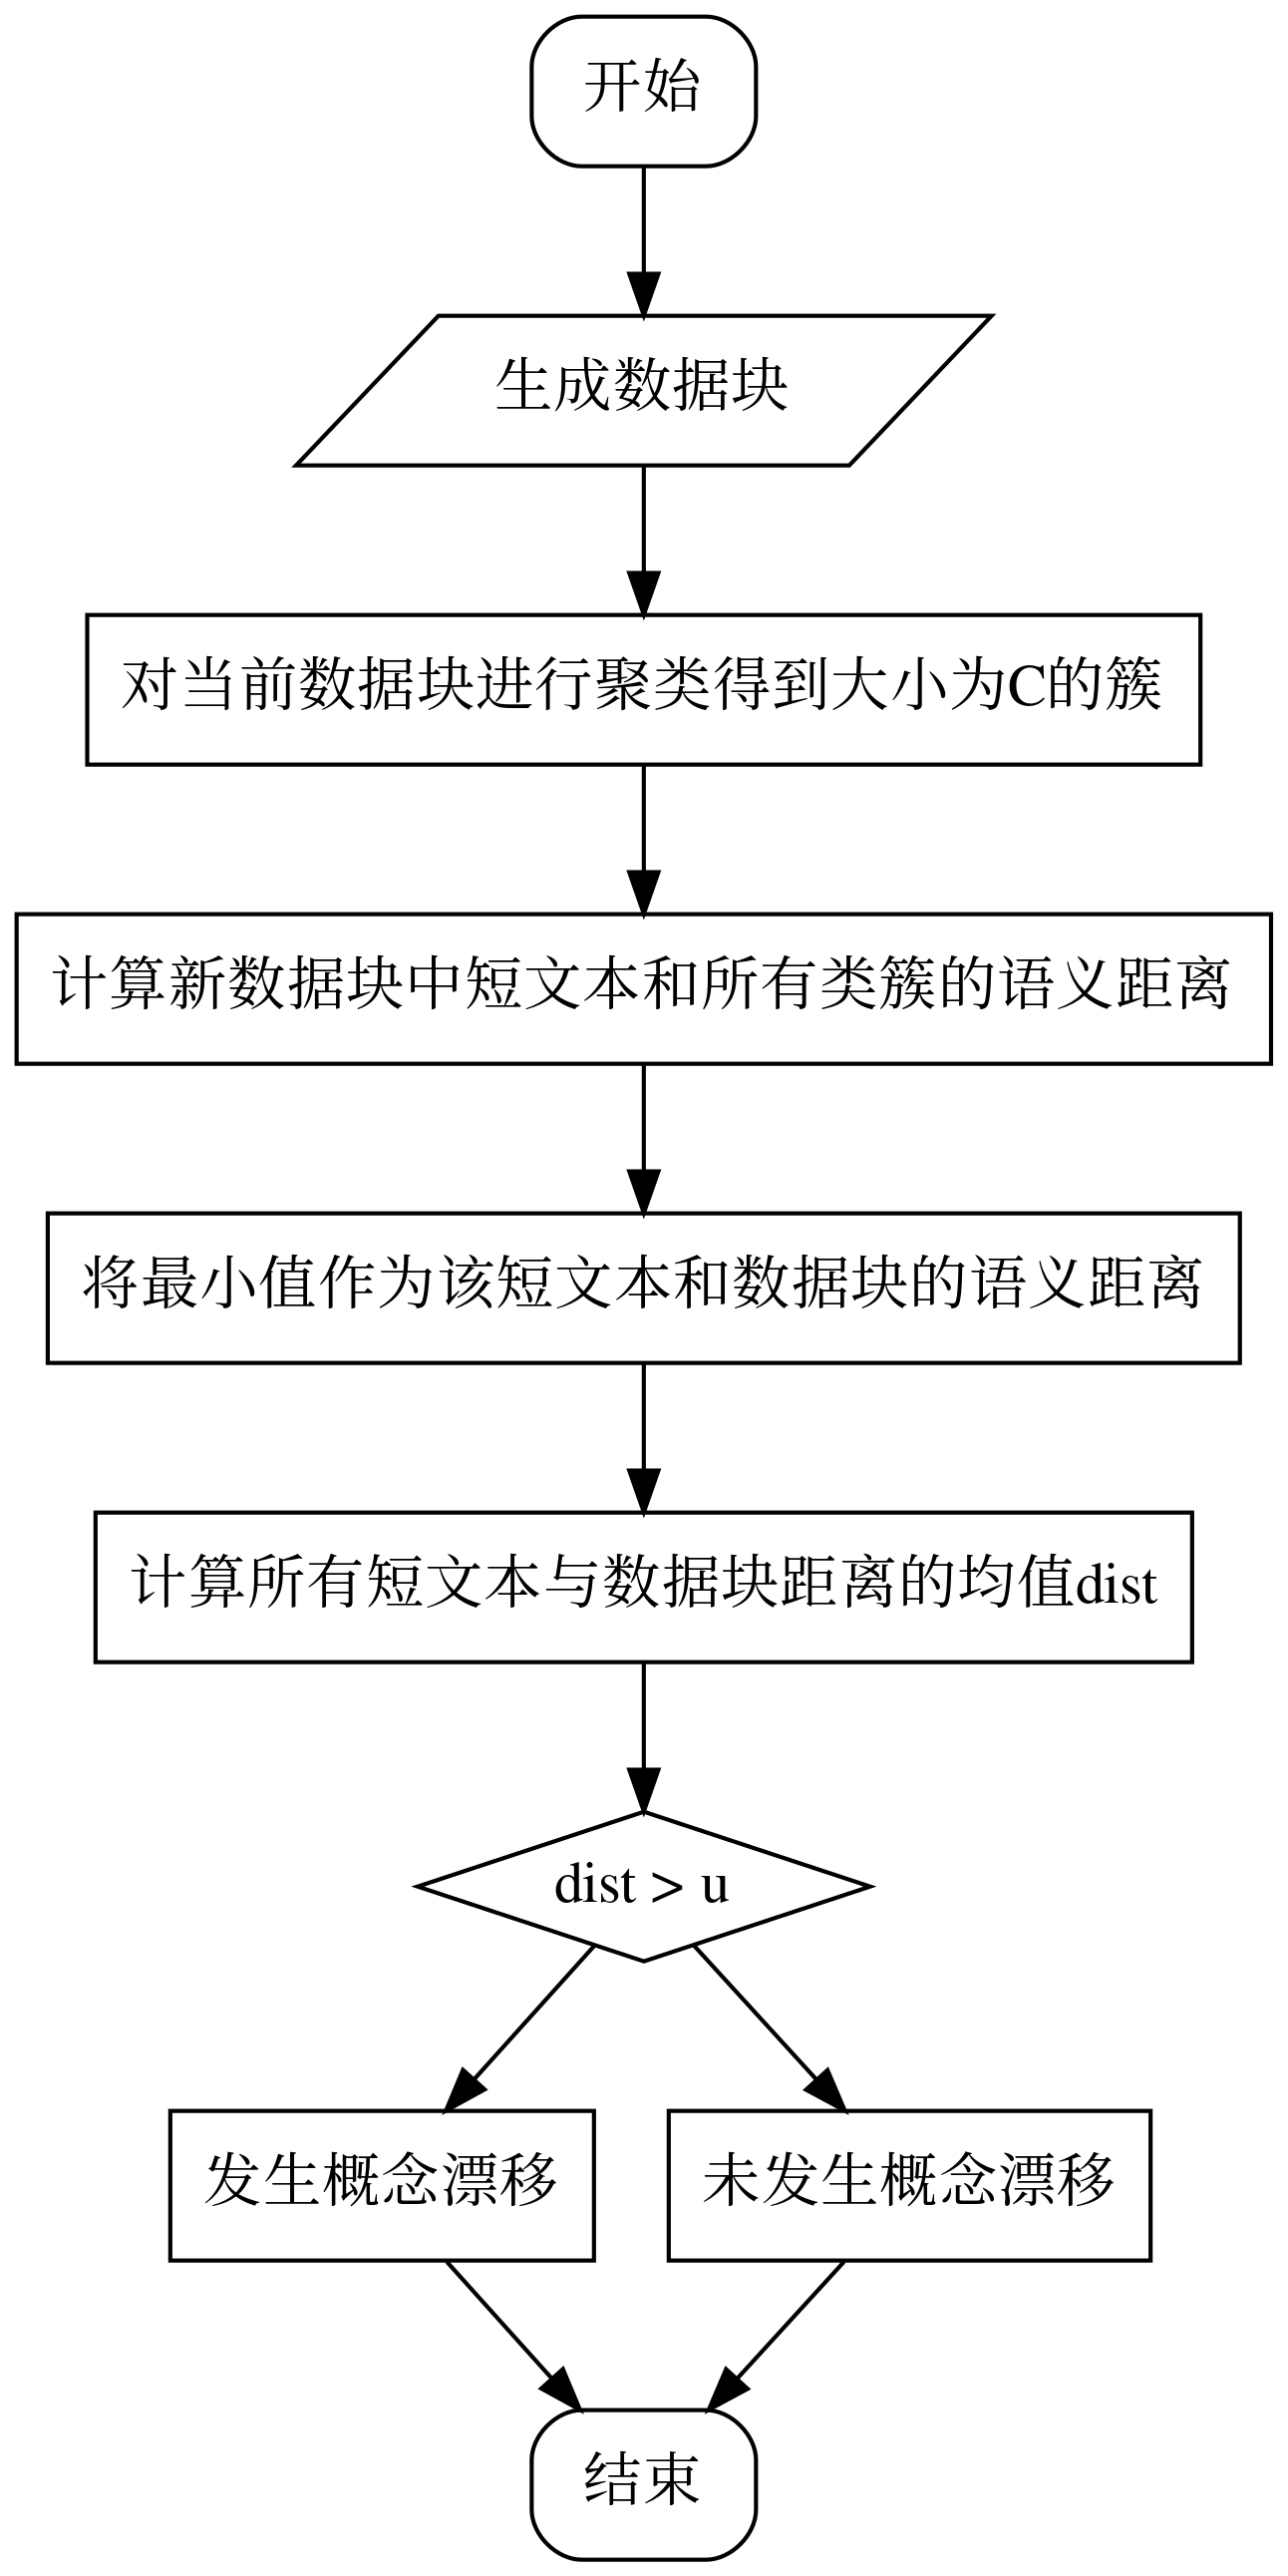
\includegraphics[width=0.4\textwidth]{concept-drift}
  \caption{概念漂移检测流程图}
  \label{fig:concept-drift}
\end{figure}

若某个类簇中的短文本数量很少,在计算两个短文本之间的语义距离$dist(d_j^{''},d_l^{''})$时便
会产生误差,由此对该项增加权重,如公式\ref{eq:dist3}:
\begin{equation}
  \label{eq:dist3}
   dist(d_j^{''},d_l^{''})=1-|I_c|/|D_i^{''}|cos(d_j^{''},d_l^{''})
 \end{equation}
 
其中,$cos(d_j^{''},d_l^{''})$为文本的余弦距离。

% \begin{equation}
%   \label{eq:cos}
% cos(d_j^{''},d_l^{''})=(z_{j,1}\cdot z_{l,1}+…+z_{j,K} \cdot
% z_{l,K})/\sqrt(\sum_{k=1}^{K}(z_{j,k})^2) \cdot\sqrt( \sum_{k=1}^{K}(z_{l,k})^2 )
% \end{equation}

最后,根据阈值u去判断是否发生概念漂移。如果$dist(D_{i+1}^{''},D_i^{''}) \in (u,1]$,则
认为数据块$D_{(i+1)}^{''}$发生了概念漂移。

\section{集成模型的构建与更新}
本章是算法的核心,构建并更新集成模型,用于预测未知标签的短文本数据。选择H个上述的数据块用于
构建SVM基分类器。当新的块$D_e$到来时,首先对它进行文本扩展和特征表示,然后使用BTM主题模型将其表示为一组主
题$D_e^{''}$。构建集成模型之前,要计算短文本$d_j^{''}$相对基
分类器的${f_h}$的权值$w_{h,j}$:

\begin{equation}
  \label{eq:w}
W_{h,j}  = (1-dist(d_j^{''},D_h^{''})) * (1-dist(D_e^{''}, D_h^{''}))
\end{equation}

其中,$1-dist(d_j^{''},D_h^{''})$表示数据块$D_e^{''}$和短文本$d_j^{''}$数据块$D_h^{''}$的语义相似度,$1-dist(D_e^{''},D_h^{''})$表示新数据块$D_e^{''}$和当前数据块$D_h^{''}$之间的语义相似度,用于减少概念漂移对准确率的影响。

下面是更新集成模型E的步骤,首先计算新数据块$D_e^{''}$和集成模型中每个旧数据块之间的语义距
离,并将新数据块构建一个分类器$f$。如果数据块$D_e^{''}$相对于E中的每个分类器都发生了概念漂
移,并且E中基分类器数量未满(即小于H),则将f添加到集成模型E中,如果E中基分类器数量已满,
则替换E中最老的基分类器。否则,将分类器f替换E中与其语义距离最小的基分类器。

% \begin{algorithm}[H]
% 	\renewcommand{\algorithmicrequire}{\textbf{输入:}}
% 	\renewcommand{\algorithmicensure}{\textbf{输出:}}
% 	\caption{集成模型更新与构建}
% 	\label{alg:ensemble}
% 	\begin{algorithmic}[1]
% 		\REQUIRE 文本数据 D,数据块 $D_e$,LDA 主题模型 $M_{LDA}$,BTM主题模型$M_{BTM}$,集成模型 E, 数
%         据块大小 H
% 		\ENSURE 数据流 S, 概念漂移检测阈值 $\mu$
% 		\STATE 利用$M_{LDA}$进行语义扩展,将$D_e$扩展为$D_e^{'}$
% 		\STATE 利用$M_{BTM}$进行特征表示,将$D_e^{'}$ 表示为 $D_e^{''}$
%         \FOR{$D_h^{''}$ in S}
%         \STATE 计算新数据块$D_e^{''}$和$D_h^{''}$的语义距离
%         \STATE 将新数据块$D_e^{''}$构建一个SVM分类器$f_e$
% 		\ENDFOR
%         \IF {数据块$D_e^{''}$相对于E中的每个分类器都发生了概念漂
%           移 \textbf{and} E中基分类器数量 < H}
%         \STATE 将f添加到集成模型E中
%         \ENDIF
%   \end{algorithmic}  
% \end{algorithm}

  \begin{algorithm}[H]
	\renewcommand{\algorithmicrequire}{\textbf{输入:}}
	\renewcommand{\algorithmicensure}{\textbf{输出:}}
	\caption{集成模型更新与构建}
	\label{alg:ensemble}
	\begin{algorithmic}[1]

		\REQUIRE 未到达数据块 D,LDA 主题模型 $M_{LDA}$,BTM主题模型$M_{BTM}$
		\ENSURE 数据流 S,集成模型 E,概念漂移检测阈值 $\mu$
		\FOR{$D_e$ in D}
		\STATE 利用$M_{LDA}$进行语义扩展,将$D_e$扩展为$D_e^{'}$
		\STATE 利用$M_{BTM}$进行特征表示,将$D_e^{'}$ 表示为 $D_e^{''}$
        \FOR{$D_h^{''}$ in $S$}
         \FOR{$d_j^{''}$ in $D_e^{''}$}
        \STATE  计算短文本 $d_j^{''}$ 和旧数据块 $D_h^{''}$ 的语义距离(公式\ref{eq:dist2})
        \ENDFOR
        \STATE 计算新数据块$D_e^{''}$ 和 旧数据块$D_h^{''}$ 的语义距离(公式\ref{eq:dist1})
         \ENDFOR
          \FOR{$d_j^{''}$ in $D_e^{''}$}
          \STATE 计算基分类器权重(公式\ref{eq:w})          
          \STATE  使用集成模型预测新数据块中的短文本 $d_j^{''}$ (公式\ref{eq:predict})
          \ENDFOR
          \STATE 计算$D_e^{''}$ 和 S 中每个块的语义距离,并根据阈值$u$判断是否发生了概念漂移
          \STATE 使用数据块 $D_e^{''}$ 训练新的基分类器$f$,并根据概念漂移的结果更新集成模型
		\ENDFOR
	\end{algorithmic}  
  \end{algorithm}


% \begin{algorithm}[H]
% 	\renewcommand{\algorithmicrequire}{\textbf{输入:}}
% 	\renewcommand{\algorithmicensure}{\textbf{输出:}}
% 	\caption{集成模型更新与构建}
% 	\label{alg:ensemble}
% 	\begin{algorithmic}[1]

% 		\REQUIRE 文本数据 D,数据块 $D_e$,LDA 主题模型 $M_{LDA}$,BTM主题模型$M_{BTM}$,集成模型 E, 数
%         据块大小 H
% 		\ENSURE 数据流 S, 概念漂移检测阈值 $\mu$
% 		\FOR{$D_e$ in D}
% 		\STATE 利用$M_{LDA}$进行语义扩展,将$D_e$扩展为$D_e^{'}$
% 		\STATE 利用$M_{BTM}$进行特征表示,将$D_e^{'}$ 表示为 $D_e^{''}$
%         \FOR{$D_h^{''}$ in $S$}
%          \FOR{$d_j^{''}$ in $D_e^{''}$}
%         \STATE  使用公式\ref{eq:dist2}计算 $d_j^{''}$ 和 $D_h^{''}$ 的语义距离
%         \ENDFOR
%         \STATE 使用公式\ref{eq:dist1}计算 $D_e^{''}$ 和$D_h^{''}$ 的语义距离
%          \ENDFOR
%           \FOR{$d_j^{''}$ in $D_e^{''}$}
%           \STATE 使用公式\ref{eq:w}计算基分类器权重          
%           \STATE  使用集成模型预测 $d_j^{''}$ 
%           \ENDFOR
%           \STATE 计算$D_e^{''}$ 和 S 中每个块的语义距离,并根据阈值$u$判断是否发生了概念漂移
%           \STATE 使用数据块 $D_e^{''}$ 训练新的基分类器$f$,并根据概念漂移的结果更新集成模型
% 		\ENDFOR
% 	\end{algorithmic}  
%   \end{algorithm}

% \begin{algorithm}
% 	\renewcommand{\algorithmicrequire}{\textbf{Input:}}
% 	\renewcommand{\algorithmicensure}{\textbf{Output:}}
% 	\caption{Ensemble Algorithm}
% 	\label{alg:1}
% 	\begin{algorithmic}[1]
% 		\REQUIRE String data D, the LDA topic model $M_{LDA}$, the ensemble model E, the set of H data;
% 		\ENSURE chunks used for the ensemble model S, the threshold $\mu$;
% 		\FOR{each data chunk $D_e$ in D}
% 		\STATE Expand $D_e$ with the topic model $M_{LDA}$ as $D_e^{'}$;
% 		\STATE Represent expaned $D_e^{'}$ as $D_e^{''}$ using BTM;
%         \FOR{$D_i^{''}$ in $S$}
%          \FOR{$d_i^{''}$ in $D_e^{''}$}
%         \STATE  Calculate semantic distance between $d_j^{''}$ and $D_i^{''}$ using \ref{eq:dist2}
%         \ENDFOR
%         \STATE Calculate semantic distance between $D_e^{''}$ and $D_i^{''}$ using \ref{eq:dist1}
%          \ENDFOR
%           \FOR{$d_i^{''}$ in $D_e^{''}$}
%           \STATE Calculate weights using \ref{eq:w}
%           \STATE  Predict $d_j^{''}$ according to ensemble model E using \ref{eq:1}
%           \ENDFOR
%           \STATE Detect concept drifts between $D_e^{''}$ and each data chunk in S
%           according to the threshold $\mu$;
%           \STATE Build a new classifier $f$ on $D_e^{''}$ and update ensemble model E according to results of concept drifts;
% 		\ENDFOR
% 	\end{algorithmic}  
%   \end{algorithm}

  
% \begin{algorithm}
% \caption{Ensemble Algorithm}
% \hspace*{0.02in} {\bf Input:} %算法的输入,
% % String data D, the LDA topic model $M_{LDA}$, the ensemble model E, the set of H data
% % \\
% \hspace*{0.02in} {\bf Output:} %算法的结果输出
% %updated E, predicted lables in data chunk $D_e$;
% \label{alg:Ensemble}
% \begin{algorithmic}

% % \For{} % For 语句,需要和EndFor对应
% % 
% %\EndFor
% \end{algorithmic}
% \end{algorithm}

% \section{实验结果和分析}

% \subsection{实验数据和评价指标}

% \subsection{基准方法和参数设置}

% \subsection{性能分析}

\section{本章小结}
本章主要介绍了本文核心算法的技术细节,提出一种带漂移检测的短文本分类算法,给出了算法的数学推导以
及运作流程。首先说明了数据集的来源,给出了短文本数据流分类的问题定义。通过Wikipedia将短文
本数据进行扩展并用BTM模型表示成主题,将数据流分块形成多个基分类器,构建集成模型,并进行了概念漂移的检
测,得到一个可用的集成分类模型,用于新数据的预测。

 % 集成分类算法研究
\chapter{算法整合与数据挖掘平台实现}

本章将在上一章节提出的短文本数据流集成分类算法的基础上,设计一个用户友好、逻辑清晰、运行高
效的面向社交网络数据的Web数据挖掘
平台。该平台基于Django 网络应用程序开发框架,整合数据挖掘算法,提供可视化的前端界面。在该
平台的设计中,使用了较为流行的MVC开发模式,使得前后端分离,这样组织的代码结构清晰,易于后
期维护
和功能拓展,提高代码运行效率。

\section{面向社交网络的数据挖掘平台设计}

在对“面向社交网络的数据挖掘平台设计”的软件进行设计时,需按照软件工程的开发流程完成。软件设计包括对软
件进行需求分析、功能设计、架构设计、API设计和服务器部署设计。软件设计是开发中的最重要一环,
也是优秀开发者必须进行的工作。“面向社交网络的数据挖掘平台设计”解决的是“怎样做”的问题。开发
的软件系统满足可用性和稳定性要求,还需对后续扩展维护提供便利。

\subsection{系统设计目标}
本系统核心算法使用SVM作为基分类器,将数据流进行分块,并考虑到对概念漂移的检测,构建高效可
用的集成学
习模型。本文事先使用Twitter API抓取推文数据,对算法进行测试,测试结果表明该算法具有良好的
拟合能力,能够对文本主题实时分类和追踪。接着,在此算法的基础之上,本文构建了一个的可视化的数据挖掘平台,将文本挖掘的一般步骤UI化,使其能更
好与用户进行交互,达到功能可复用、可交互的目的。
本系统的技术栈是Python+Scikit-Learn+Django+MongoDB ,它集成了数据上传、数据预处理与清洗、数据建模、数据可视
化等常用的数据挖掘技术,使得用户无需了解算法和数据挖掘技术内部的运行机制,即可完成对数据的
分析工作。同时,该系统考虑到扩展性问题,当新的数据挖掘算法被提出时,也可以很方便地进行整合。

\subsection{系统架构设计}
根据本系统的设计目标,将其划分4个模块,分别是数据上传、数据预处理、主题跟踪和数据可视化。
图\ref{fig:platform}是本系统的整体架构图:

\begin{figure}
  \centering
  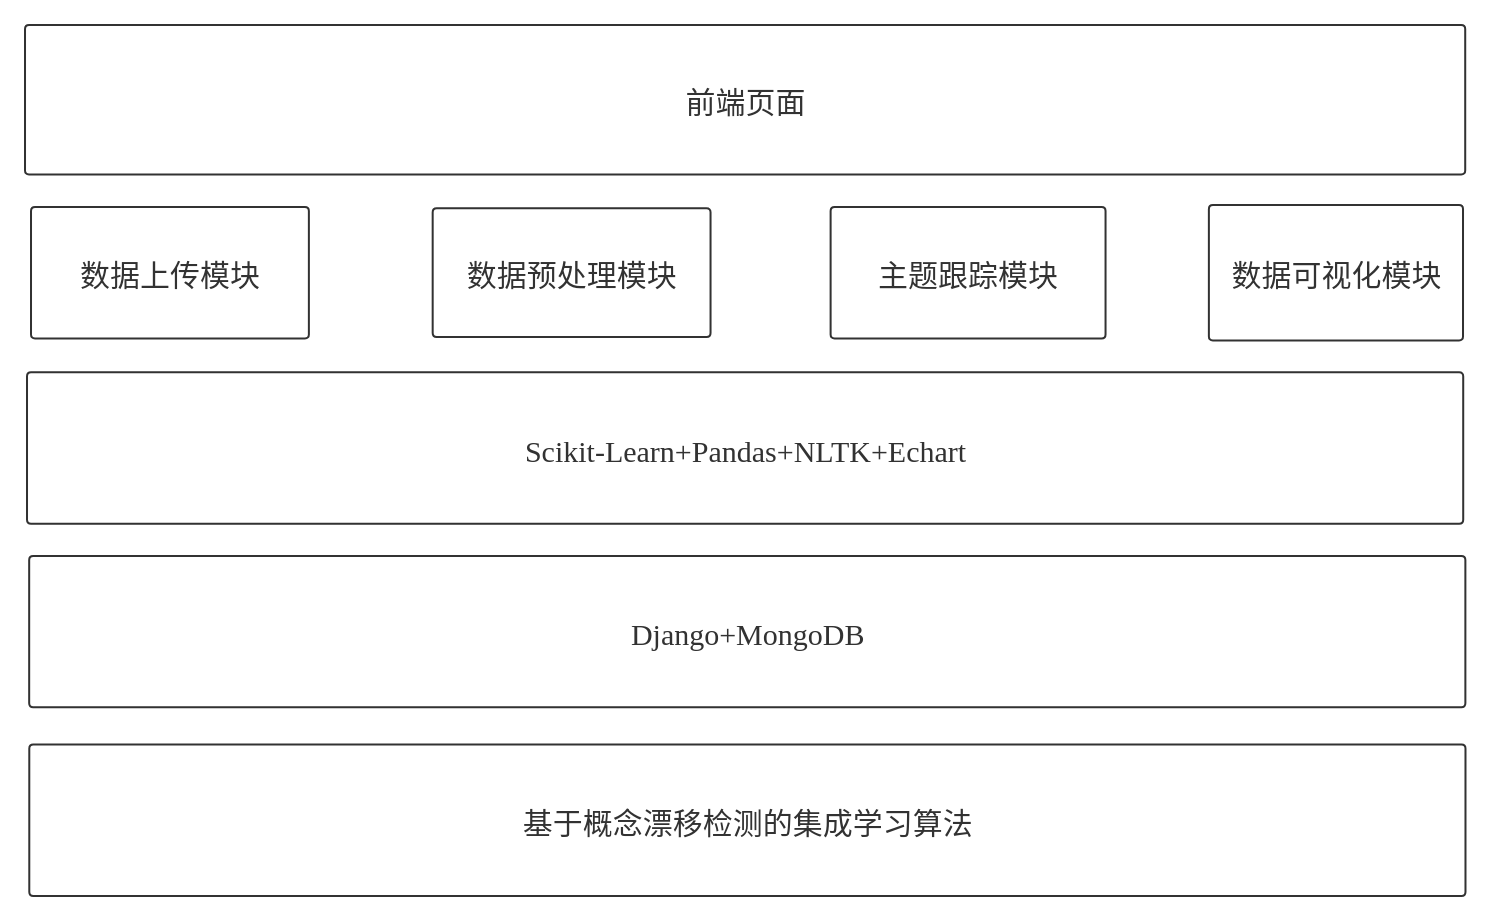
\includegraphics[width=1.0\textwidth]{platform}
  \caption{数据挖掘可视化平台架构图}
  \label{fig:platform}
\end{figure}

本文采用MongoDB作为数据库,由于着重于算法研究,本文数据库较为简单,只有数据内容、数据标签
和时间等项。

\subsection{系统功能模块}
系统的功能模块主要包含四个部分,分别是:数据上传模块、数据预处理模块、主题跟踪模块和数据可
视化模块。各个模块的主要功能如下:
\begin{description}
\item [数据上传:]用于将本地的数据文件导入到MongoDB中;
\item [数据预处理:]负责对上传后的文档进行去停用词、词干提取、词形转换、去噪等操作;
\item [主题跟踪:]本平台的核心模块,是集成学习的算法整合;
\item [数据可视化:]对数据和主题跟踪结果进行了图表展示;
\end{description}

\section{系统实现}

\subsection{软硬件环境}
本次实验的所有模型框架均在python3.6上运行,为保证代码运行稳定、高效,基于Scikit-Learn机器
学习框架进行二次开发,它的特点是可以快速实现研究人员的想法而不拘泥于模型细节。平台运行环境
分本地环境和服务器端环境。本地用于算法的实现与测试,服务器端用于部署整合算法的Django服务。

\begin{table}[H]
  \begin{singlespace}
    \renewcommand{\arraystretch}{1.5} %控制行高
    \centering\caption{软硬件环境}\label{tab:env}                              
    \begin{tabular}{cl}\hline
      环境 & 硬件信息 \\ \hline                                                
      \verb|本地环境| & 操作系统: Debian 10 Testing 版 \\
           & CPU:Intel Core i5 5300U 2.3GHz \\
           & RAM:8.00GB \\
           & 显卡:Intel(R)HD Graphics 630(1024MB)  \\      
           & 硬盘:NVMe SAMSUNG MZVLW128(128GB)+1T机械硬盘 \\ \hline
      \verb|服务器环境(阿里云计算平台)| & 操作系统: Debian 9 Stable版 \\
           & CPU:1.0GHz \\
           & RAM:2.00GB \\
           & 带宽:2M \\ \hline
    \end{tabular}                                                              
  \end{singlespace}                                                            \end{table}               

% \subsection{实验数据集}
% 本文数据通过借助Twitter官方提供的“关键字”API进行采集。一共爬取了从2011年11月到2013年1月的
% 5个类别的共约6万条数据。

\subsection{数据上传模块}
数据上传模块主要用于上传本地文件到数据库中,用户通过在前端页面点击“文件路径”按钮,即触发文
件上传控件,用户通过弹出的文件目录浏览功能访问本地文件,选中后既可获得文件路径,并会自动填
充文件名到“数据集标签”中。

本地文件格式为\texttt{.csv},文件名即为类标签,文件的每一行代表一条推文数据,每一列为该推文的属性,其中包括发布人TwitterID、是否转推、发布时间、推文内容等。由于本文并不需要所有属性,数据上传时就需先对需要的文本进行提取,保留发布人时间、正文内容以及类标签。图\ref{fig:upload}是数据上传模块参数设置。

\begin{figure}[htb]
  \centering
  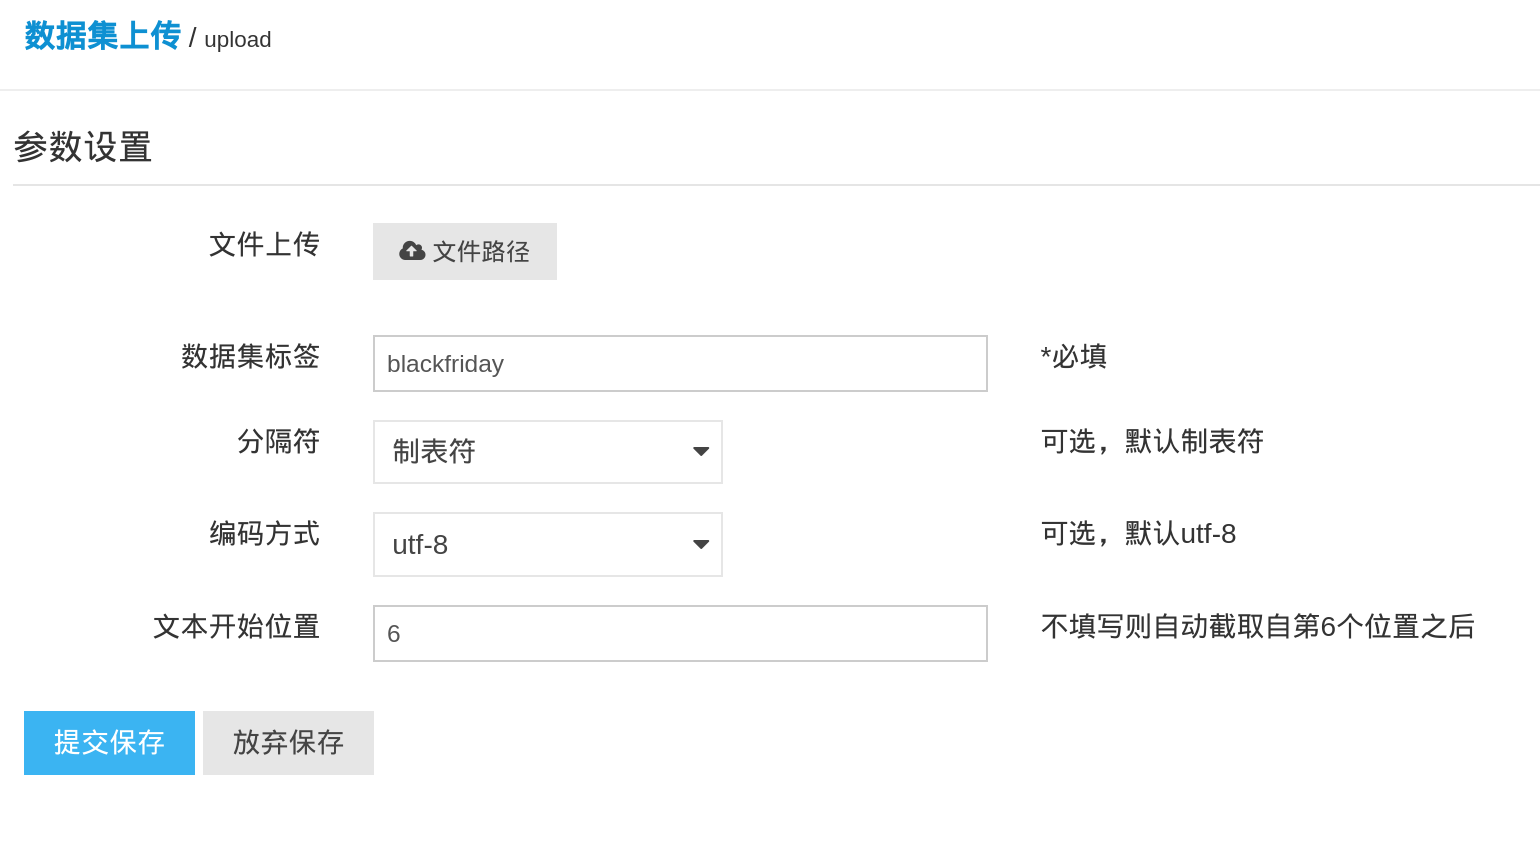
\includegraphics[width=0.8\textwidth]{upload}
  \caption{数据上传参数设置}
  \label{fig:upload}
\end{figure}

设置好其他参数分割符、编码方式、文本开始位置等后,点击提交保存,前端Javascript就会发起ajax请求,django接受到请求后,url机制会匹配到对于视图模块,调用相应的方法,对数据进行保存。

\begin{minted}{py}
urlpatterns = [
    re_path(r'^$', upload),
    re_path(r'uploadfile', upload_file)
]
\end{minted}


\begin{figure}[H]
  \centering
  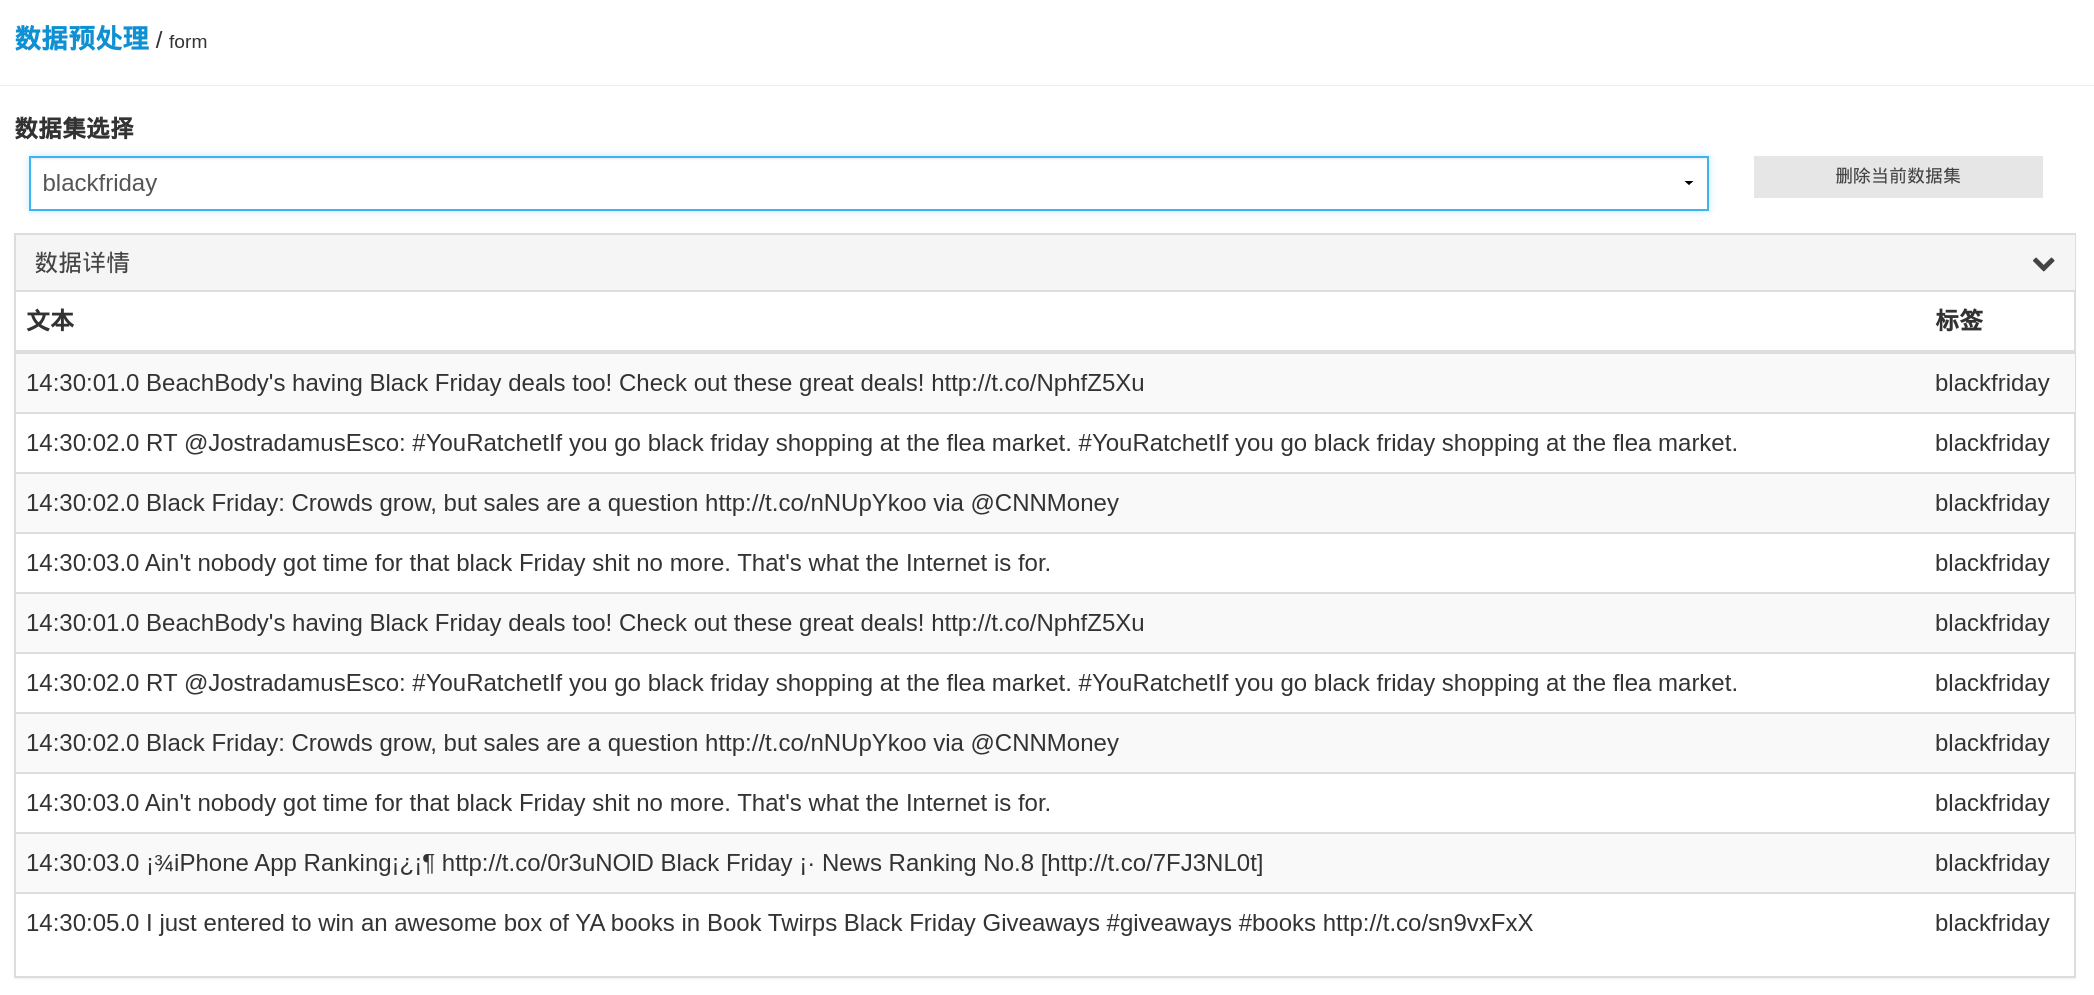
\includegraphics[width=0.8\textwidth]{upload_data}
  \caption{上传数据展示}
  \label{fig:upload_data}
\end{figure}

图\ref{fig:upload_data}是上传后的数据集blackfriday。

\par\subsection{数据预处理模块}
数据预处理模块用于负责对上传后的文档进行去停用词、词干提取、词形转换、去噪等操作。用户在前
端页面选好需要处理的一类文档,选择停用词词库,询问是否进行词干提取、词形转换、大小写转换,
自定义正则表达式等。图\ref{fig:preprocessing}为数据预处理模块的参数设置。

\begin{figure}[H]
  \centering
  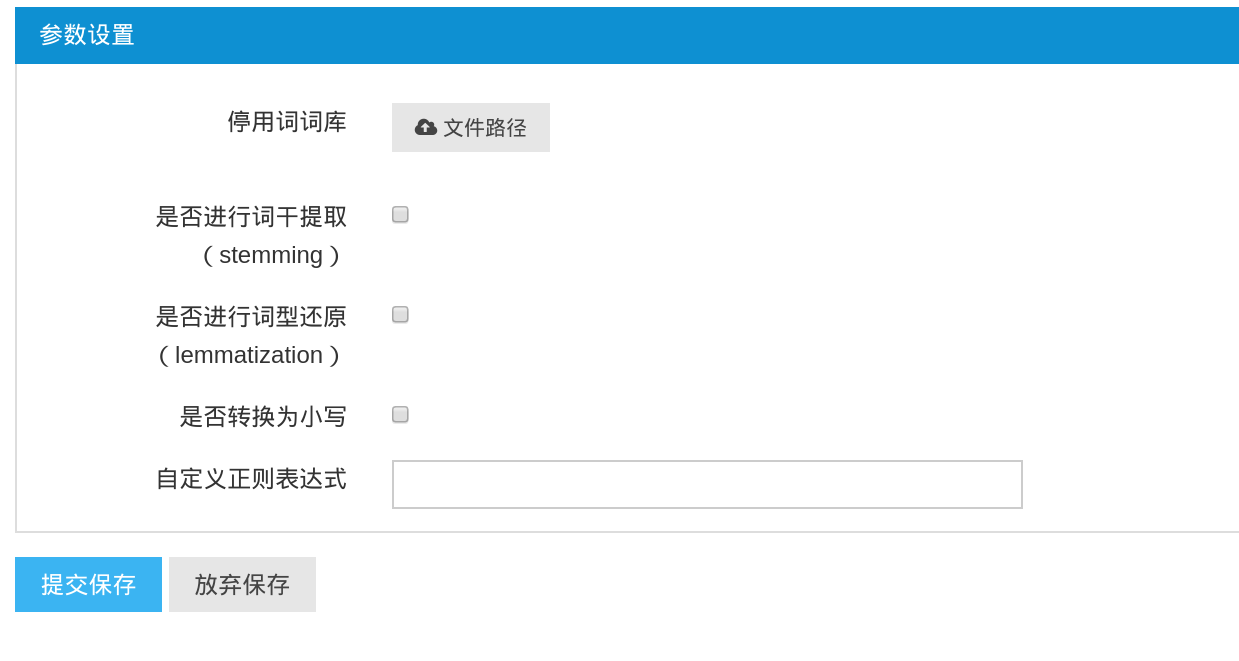
\includegraphics[width=0.8\textwidth]{preprocessing}
  \caption{数据预处理参数设置}
  \label{fig:preprocessing}
\end{figure}

用户点击“提交保存”后,前端Javascript发起ajax POST请求,url路由匹配到相应的视图并进行函数调
用,对选中的文本数据集进行数据预处理。通过ORM条件查询获得表单对象,遍历该对象中的文本,借
助的预处理函数完成数据预处理的一系列操作。下面是视图views.py中的接受处理请求的部分代码:

\begin{minted}{py}
@csrf_exempt
def startProcess(request):
    try:
        if request.method == 'POST':
            # 接受前端Post请求    
            label = request.POST['label']
            ... ...
            # ORM查询符合条件的数据集
            dataset = DataModel.objects.filter(label=label)
            # 进行文本预处理
            if handleProcess(dataset, stopwords, regex):
                status = "text preprocessing success!"
            else:
                status = "sorry, text preprocessing fail."
            response = {"status": status}
            return HttpResponse(json.dumps(response), content_type='application/json')
    except Exception as e:
        print(e)
\end{minted}

\subsection{主题跟踪模块}
该模块是本系统的核心模块,整合第三章提出的集成学习算法,采用用户上传的数据模拟数据流,进行
主题跟踪。用户上传数据后,调用预处理模块对文档进行文本预处理,借助外部语料库对文本进行语料
扩展,并完成特征表示,得到每个文档的的文档-主题矩阵,即可放入集成模型进行训练,该模块能够
实时监控训练过程,展示集成模型的日志输出情况,同时可视化地显示BTM提取到的主题分布。

用户需预设数据块大小、数据块数量以及概念漂移的阈值,同时用户可以调整BTM主题模型的参
数,选择合适的主题值和迭代次数,调整SVM的参数,采用核函数类型、核函数系数Gamma以及惩罚系数
C。图\ref{fig:topic}是主题跟踪模块的参数设置。

\begin{figure}[H]
  \centering
  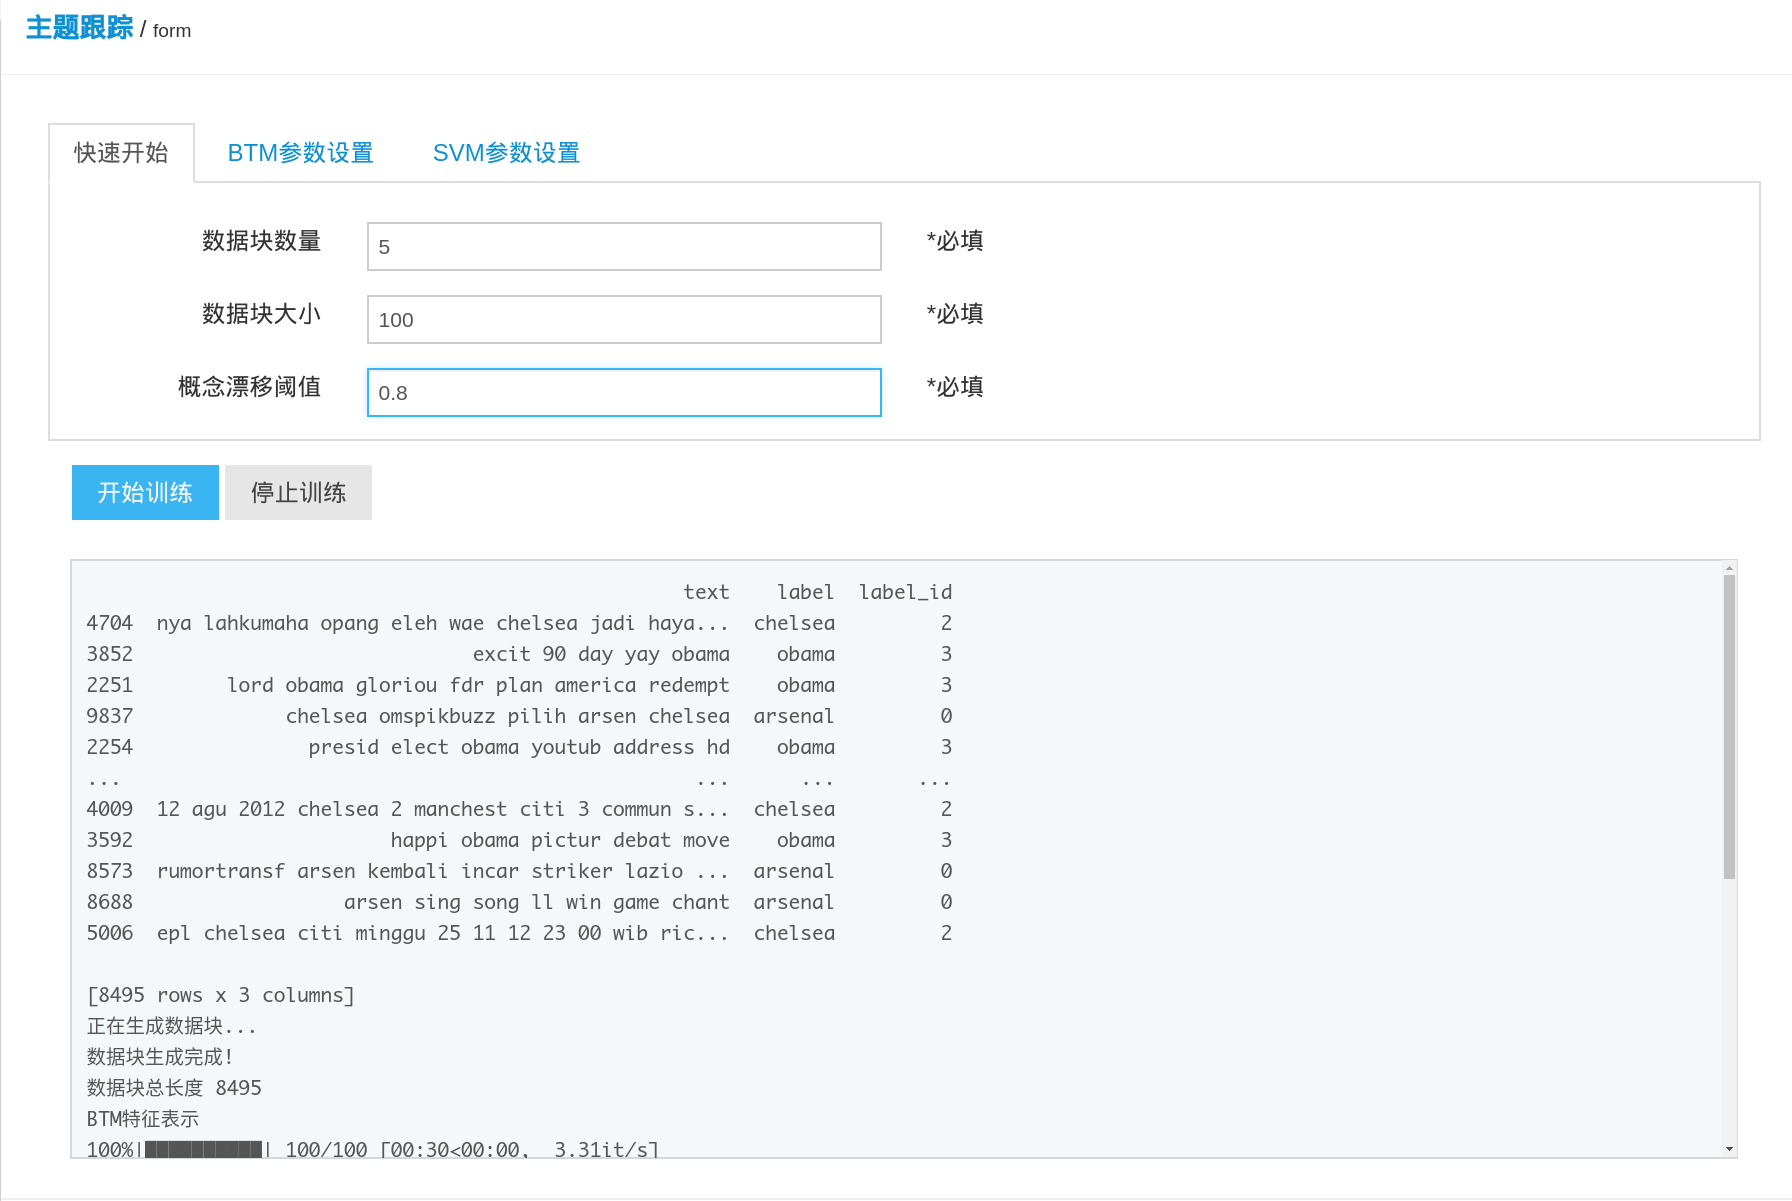
\includegraphics[width=1.0\textwidth]{topic}
  \caption{主题跟踪模块}
  \label{fig:topic}
\end{figure}

用户设置好参数后,点击“开始训练”,前端即发起请求,后端URL将请求进行分发,调用
topicProcess()函数进行主题跟踪,该函数会将数据库中的数据读出,放入一个Pandas的dataframe对象
中并打乱,用于模拟数据流,接着数据流被分块传入集成模型中进行训练,动态更新集成模型。前端通过Websocket建立长连接,
实时将训练日志输出到前端页面中,并展示主题的追踪结果。

该模块的URL路由:
\begin{minted}{py}
urlpatterns = [
    re_path('^$', topic),
    re_path('topicProcess', topicProcess)
]
\end{minted}

主题跟踪模块视图函数:
\begin{minted}{py}
@csrf_exempt
def topicProcess(request):
    try:
        if request.method == 'POST':
            # 获取前端传入参数
            H = int(request.POST['H'])
            blocksize = int(request.POST['blocksize'])
            u = float(request.POST['u'])
            ... ...
            # 获取数据流
            for label in labels_:
                query = DataModel.objects.filter(label=label)
                for row in query:
                    texts.append(row.text)
                    labels.append(row.label)
            ... ...
            data.dropna(axis=0, how='any', inplace=True)
            data = shuffle(data)
            # 初始化集成模型
            E = Ensemble(H = H, blocksize = blocksize, u = u,
            base = "svm", K = K, btm_iterations = iter,
            svm_gamma = "auto", svm_C = C, svm_kernel = "linear")
            # 集成模型训练              
            E.fit(data.text, data.label_id)
            ... ...
    except Exception as e:
        print(e)
\end{minted}

% 为了更加方便地对数据流进行操作,使用Python面向对象编程,将数据流抽象成为了数据块类Block,
% 并使用迭代器实现了对数据块的实时生成。

% 做好上述的准备工作后,即可将对带有类标签数据通过Block的形式传入集成学习模型中进行模型训练与更新,最后得到一组大小为H的基分类器集,使用得到的模型即可完成对未知标签数据进行预测和主题分析。

% 下面是整个算法的测试代码(考虑篇幅,已简化部分代码):
% \begin{minted}{py}
%     from sklearn.model_selection import train_test_split
%     from sklearn import preprocessing
%     from sklearn.feature_extraction.text import TfidfVectorizer

%     # 通过ORM模型从数据库读出数据,保存到textDF数据结构中;
%     query = DataModel.objects.all()
%     textDF = pandas.DataFrame()
    
%     ......

%     # 分割数据集,并提取TF-IDF值;
%     X_train, X_test, y_train, y_test = train_test_split(textDF.text, textDF.label, test_size=0.25, random_state=23)
%     vec_tfidf = TfidfVectorizer()
%     vec_tfidf_f = vec_tfidf.fit(X_train)
%     train_dtm_ngram = vec_tfidf_f.transform(X_train).toarray()
%     test_dtm_ngram = vec_tfidf_f.transform(X_test).toarray()
    
%     # 对标签进行向量化编码;
%     encoder = preprocessing.LabelEncoder()
%     y_train = encoder.fit_transform(y_train)
%     y_test = encoder.fit_transform(y_test)
    
%     # 使用Ensemble进行分类测试;
%     E = Ensemble(H=10, blocksize=100)
%     a = train_dtm_ngram[0]

%     # 对数据流生成数据块,并通过定义生成器生成测试数据;
%     f = E.gen_blocks(test_dtm_ngram, y_test)
%     block = next(f)
%     test_x = block.getX()
%     test_y = block.getY()

%     # 集成模型的训练;
%     E.fit(train_dtm_ngram, y_train)
%     y_pred = E.predict(test_x)
    
%     from sklearn import metrics
%     from sklearn.metrics import classification_report

%     # 分类评价指标;
%     recall = metrics.recall_score(test_y, y_pred)
%     F1 = metrics.f1_score(test_y, y_pred)
%     print("正确率:", np.mean(y_pred == test_y))
%     print("召回率:", recall)
%     print("F1:", F1)

%     # 打印评价报告;
%     target_names = ['obama', 'smartphone']
%     print(classification_report(test_y, y_pred, target_names=target_names))
    
% \end{minted}

\subsection{数据可视化模块}
该模块主要用于图表的展示,使用Echart模块进行图表绘制,其中包括对源数据中的文本进行词频统计,
分别统计数据集中每个类簇的文本总数,生成条形图和饼状图。统计每个文档的长度,使用折线图表示
各长度文档出现的频率,可以很清楚的发现,长度在40左右的文档最多,这符合社交网络中文本的特征。使用主题模型分析文本数据,通过设置主题数,对文本进行主题划分,得到主题分布图。

\begin{figure}[H]
  \centering
  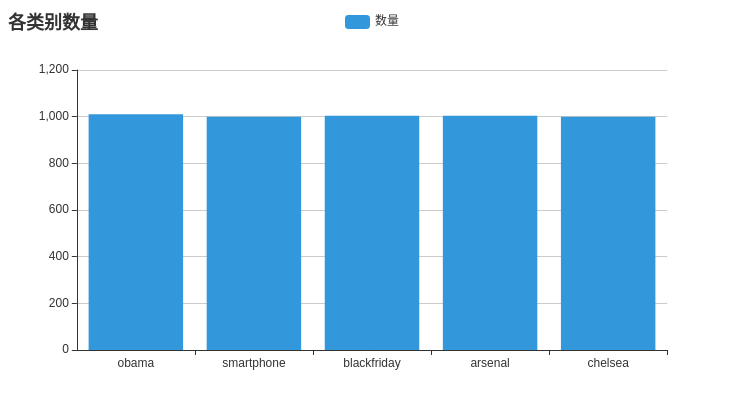
\includegraphics[width=1.0\textwidth]{fig1}
  \caption{各类别数量图}
  \label{fig:upload}
\end{figure}

\begin{figure}[H]
  \centering
  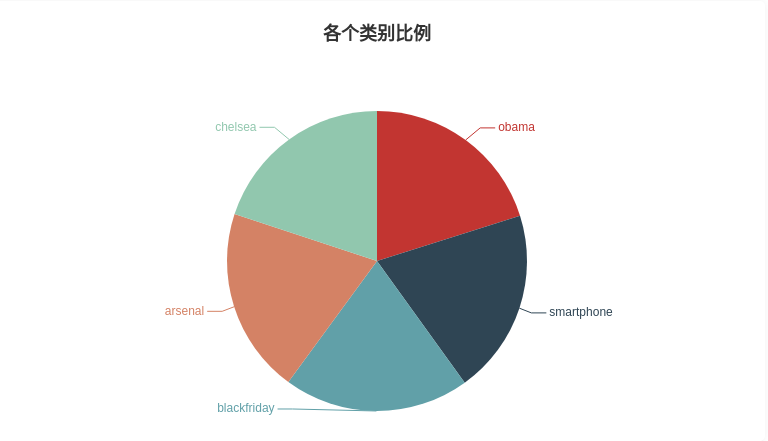
\includegraphics[width=1.0\textwidth]{fig2}
  \caption{各类别比例图}
  \label{fig:upload}
\end{figure}

\begin{figure}[H]
  \centering
  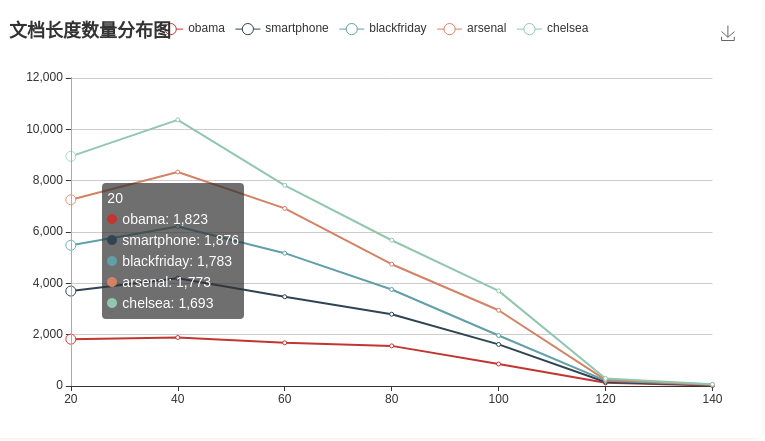
\includegraphics[width=1.0\textwidth]{fig3}
  \caption{文档长度数量分布图}
  \label{fig:upload}
\end{figure}

% \subsection{应用案例}

\section{本章小结}
本章主要介绍了Twitter数据挖掘可视化平台的搭建,使用的技术包括但不限于Django开发框架、
Scikit-learn、pandas、numpy、echart、mongodb等。以Django框架为Web平台主体,使用Scikit-learn
进行算法实现,完成了整个平台的技术整合。实现的功能模块包括:数据上传、数据预处理、数据可视
化、主题跟踪等。将数据挖掘中需要使用到的如数据预处理与数据清洗、特
征提取、分
类算法应用等过程UI化,大大降低了使用者的门槛。同时,也使研究人员能及时、快速发现研究中的问
题,具有较高的应用价值。


 % 算法与系统实现
% \chapter{测试与展示}

\section{测试环境}

\section{测试过程}

\section{平台展示}

\section{本章小结}



 % 测试与结论

\chapter{总结与展望}

\section{工作总结}
当下,随着信息与通信技术的发展,各种网络平台不断壮大,信息随时产生,海量短文本数据汇入信
息的洋流。这些数据蕴含丰富的信息,有很高的研究价值,因此高效挖掘这些数据的内涵变得愈发重要。短
文本分类工作一直是数据挖掘领域研究的热点,它有着不用一般文本数据的特点,即语义缺失、高维稀
疏等。并且,短文本数据流还会随时间迁移产生概念漂移现象。这些特点使得传统算法的对其应用的效果较差。因此,本文借助了文本扩展的方法,缓解短文本
的语义信息缺乏的问题,并提出一种基于块的集成分类模型,考虑对概念漂移的检测,对短文本数据流
分类进行了以下的研究:

1. 本文第一章介绍了短文本数据流分类的研究背景及意义,给出短文本数据流分类面临的问题和挑战,介绍国内外研究人员对短文本分类问题研究的现状,对已存在的问题提出的解决方式。接
着阐述了本文主要研究的内容,即设计一个集成分类算法和可视化的数据挖掘平台。给出论文的组织框
架,分别简要介绍了每个章节的主要内容。

2. 第二章为相关技术和理论的介绍,给出了文本挖掘的一般步
骤,包括“数据清洗与预处理”、“分词”、“特征提取”、“特征表示”、“算法应用”等。并分别就短文本分
类和短文本数据流分类介绍相关的技术。

3. 第三章为本文核心,介绍了基于概念漂移检测的短文本数据流分类算法。该算法大致思想是:通过文本扩展,缓解语义信
息缺失,借助时间序列对数据流进行块分割,对每个块训练基分类器构建集成模型,并通过计算块和块语义距离判断是
否发生了概念漂移。文本扩展使用的Wikipedia作为外部语料,借助LDA主题模型进行主题分析,通过主
题相似性进行文本扩展。

4. 第四章介绍了构建数据挖掘平台的细节,并对前面提到了基于概念漂移检测的短文本数据流分类算
法进行整合。该平台基于Django搭建,采用MVT的开发模式,前后端逻辑分离,使用Scikit-learn、
pandas、numpy、nltk等强大的数据挖掘与机器学习库,完成算法设计。

\section{工作展望}
进入大数据时代的今天,互联网中越来越多的如“Tweets”、“微博”、“新闻标题”等短文本数据,短文本
分类问题将一直将是研究的焦点。短文本数据流带来语义信息不足、特征高维稀疏等问题,本文提出借
助外部语料库扩展的方式,缓解稀疏性,实验表明具有良好的效果。同时,本文提出的数据挖掘平台当
前较为简单,经过进一步研究认为,未来还有一下几个方面的工作值得进行:

\begin{itemize}
\item 本文通过外部语料库扩展的方式缓解文本特征高维稀疏的问题,虽然方法可行,但是扩展过程较
  为耗时,考虑是否可以使用更好的方式对文本空间进行扩展。
\item 对于短文本数据流的分类问题,本实验采用的数据集较小,取得的效果无法证明实际应用大数据的
普适性,接下来需要继续研究如何将算法应用到真实的大数据集当中。
\item 数据挖掘平台的优化,文本仅应用了一种基于集成学习的分类方法到数据挖掘平台当中,在后续研究中,考虑添加更多的数据挖掘算法到平台中。同时,平台的数据需使用手动上传的方式进行模拟,未来考虑整合API或者爬虫的方式,对数据进行实时分析和预测。
\end{itemize}

总之,短文本数据流分类作为数据挖掘研究的重要方向,可以研究的内容还很多,在接下来的学习中,如何将算法真正应用到实际中,提供优雅的解决方案,始终是研究者的重要任务。 % 总结与展望

%%%%% appendix (参考文献、指导教师简介、鸣谢、附录)
\appendix % keep this line
\makebib % 参考文献

\begin{advisorInfo} % 指导教师简介
  % 张雁,女,——岁,博士,教授,毕业于——大学,——专业。现任
  % 西南林业大学大数据与智能工程学院——。执教——,有丰富的——经验。
  
\end{advisorInfo}

\begin{acknowledgment} % 致谢
完成本篇论文,意味着我的本科学习生涯就快要结束了。借此机会感谢一路上帮助、关心过我的老师、
同学和我的家人们。大数据与智能工程学院是我心中的霍格沃茨学院,四年里,每每我更加深刻地理解
计算机时,它总会让我感到犹如魔法般绚丽。正是那些理性的光辉,一次次令我着迷,让我对
这门学科的兴趣被一次次激活。

首先,由衷感谢我的毕业论文指导老师张雁教授以及合肥工业大学李培培教授,张老师学识渊博、为人正直而且平易近人,深得学生们的
爱戴与尊敬。在我完成我的毕业论文的过程中,从开题到中期报告再到论文撰写,张老师都给予了我很
大的帮助,即便疫情期间没能去到学校,张老师仍通过网络不断监督、指导着我们的学习,我们作为
学生被张老师认真负责、严谨治学的态度深深打动,时刻提醒自己今后一定要学会这种优秀的品质,做一个对社会、对国家
有价值的科研人。李老师是我未来研究生生涯的指导老师,她给了我本论文的命题和研究方向,在前
期学习、编码以及论文撰写过程中提出了许多宝贵的建议,也让我在短短几个月时间里对未来研究内容有了大致
的了解,为研究生生涯提前做好准备。

其次,感谢四年本科生涯帮助过我的其他老师们以及同学们。王晓林教授是我来到大数据与智能工程学院遇到
的第一位老师,我始终记得那个昆明独有的沁人心脾的早晨,我走进教室,终于开始了我计算机学习生涯的
第一堂课,王老师轻松幽默却又深刻的授业方式让我终身难忘,他的出现点燃我对这个学科的热情,让我
接下来能够一步一个脚印完成本科阶段的学习。当然,大数据与智能工程学院的其他各位老师也都是我学习路上的明
灯,与他们的交流过程中,我学习到的不仅仅是知识,还有如何思考问题的方式,这对我来说无疑是巨
大的收获。计算机科学与技术专业的每位同学,都有值得学习的地方,他们当中不乏有十分聪明又努力
的,也有喜欢不断追求新事物、新挑战的,他们对我的影响足以改变我的人生。

同时,感谢我的家人,因为只有他们作为我强大的后盾,让我在生活上没有后顾之忧,我才能专心下来
学习。在我遇到困难时,也是他们第一个站出来,给我支持和力量,他们是我不断前行的人生路中最大
的动力。

最后,感谢美国计算机教授高德纳(Donald Ervin Knuth)编写的功能强大的排版软件\TeX{}。感谢美国计算
机科学家莱斯利·兰波特(Leslie Lamport)教授为\TeX{}开发的简单易用的\LaTeX{}宏包。感谢
王老师编写的优秀的\LaTeX{}模板。
让在撰写毕业论文时有着非同寻常的体验,基本无需考虑繁杂的排版与格式问题,真正专注到书写论文
本身,才能更好完成这篇论文。
  
  % \cite{Wangxiaoling}
  
\end{acknowledgment}

%%%%% 附录章节
\singlespacing
\include{chapters/append} 

\end{document} % 结束。不要动下面几行!

%%% Local Variables:
%%% mode: latex
%%% TeX-master: t
%%% End:


%%% Local Variables:
%%% mode: latex
%%% TeX-master: t
%%% End:
